%%%%%%%%%%%%%%%%%%%%%%%%%%%%%%%%%%%%%%%%%%%%%%%%%%%%%%%%%%%%%%%%%%%%
%% I, the copyright holder of this work, release this work into the
%% public domain. This applies worldwide. In some countries this may
%% not be legally possible; if so: I grant anyone the right to use
%% this work for any purpose, without any conditions, unless such
%% conditions are required by law.
%%%%%%%%%%%%%%%%%%%%%%%%%%%%%%%%%%%%%%%%%%%%%%%%%%%%%%%%%%%%%%%%%%%%

\documentclass[
  digital, %% This option enables the default options for the
           %% digital version of a document. Replace with `printed`
           %% to enable the default options for the printed version
           %% of a document.
  table,   %% Causes the coloring of tables. Replace with `notable`
           %% to restore plain tables.
  lof,     %% Prints the List of Figures. Replace with `nolof` to
           %% hide the List of Figures.
  lot,     %% Prints the List of Tables. Replace with `nolot` to
           %% hide the List of Tables.
  %% More options are listed in the user guide at
  %% <http://mirrors.ctan.org/macros/latex/contrib/fithesis/guide/mu/fi.pdf>.
]{fithesis3}
%% The following section sets up the locales used in the thesis.
\usepackage[resetfonts]{cmap} %% We need to load the T2A font encoding
\usepackage[T1,T2A]{fontenc}  %% to use the Cyrillic fonts with Russian texts.
\usepackage[
  main=slovak, english, %% By using `czech` or `slovak` as the main locale
                %% instead of `english`, you can typeset the thesis
                %% in either Czech or Slovak, respectively.
  german, russian, czech %% The additional keys allow
]{babel}        %% foreign texts to be typeset as follows:
%%
%%   \begin{otherlanguage}{german}  ... \end{otherlanguage}
%%   \begin{otherlanguage}{russian} ... \end{otherlanguage}
%%   \begin{otherlanguage}{czech}   ... \end{otherlanguage}
%%   \begin{otherlanguage}{slovak}  ... \end{otherlanguage}
%%
%% For non-Latin scripts, it may be necessary to load additional
%% fonts:
\usepackage{paratype}
\def\textrussian#1{{\usefont{T2A}{PTSerif-TLF}{m}{rm}#1}}
%%
%% The following section sets up the metadata of the thesis.
\thesissetup{
    date          = \the\year/\the\month/\the\day,
    university    = mu,
    faculty       = fi,
    type          = mgr,
    author        =  Jerguš Fašánek,
    gender        = m,
    advisor       = {Ing. RNDr. Barbora Bühnová, Ph.D.},
    title         = {Cloudový slovníkový prekladač pre vývojárov},
    TeXtitle      = {Cloudový slovníkový prekladač pre vývojárov},
    keywords      = {Slovník, preklad slov, synchronizácia, cloud, Node.js, React },
    TeXkeywords   = {Slovník, preklad slov, synchronizácia, cloud, Node.js, React},
    bib           = example.bib,
}
\thesislong{abstract}{
   Cieľom diplomovej práce je navrhnúť a vytvoriť backend pre synchronizáciu slovníkov desktopovej offline aplikácie a následne vytvoriť webový frontend. Slovníky v aplikácii slúžia pre vývojárov spoločnosti Siemens, s.r.o. na zjednodušenie práce na medzinárodných projektoch v cudzích jazykoch.
}
\thesislong{thanks}{
    Rád by som sa poďakoval Mgr. Jiřímu Ohnheiserovi za pomoc a užitočné rady pri vypracovaní diplomovej práce a mojej priateľke Nikole Mišíkovej za podporu počas písania práce.
}
\usepackage{makeidx}      %% The `makeidx` package contains
\makeindex                %% helper commands for index typesetting.
%% These additional packages are used within the document:
\usepackage{paralist} %% Compact list environments
\usepackage{amsmath}  %% Mathematics
\usepackage{amsthm}
\usepackage{amsfonts}
\usepackage{url}      %% Hyperlinks
\usepackage{markdown} %% Lightweight Markup
\usepackage{listings}
\begin{document}
\chapter{Úvod}
Pri vývoji softvéru v IT spoločnostiach spoluracuje medzi sebou viacero vývojárov a často sa využívajú už existujúce zdrojové kódy, na ktorých sa ďalej pracuje. Týka sa to aj spoločnosti Siemens, ktorá bola založená v Nemecku, ale pôsobí aj v Českej republike.

Vývojári v Čechách tak spolupracujú s tými v Nemecku a pracujú s kódom, v ktorom je množstvo cudzích výrazov v nemeckom jazyku, ktoré sa však nenachádzajú v bežných prekladových slovníkoch, pretože sú veľmi špecifické a sú prispôsobené používaniu v kóde. Preto bola vytvorená desktopová aplikácia, ktorá umožňuje vytváranie vlastných slovníkov, do ktorých je možné postupne pridávať dané výrazy a k nim aj ich preklad. Nevýhodou tejto aplikácie je ale to, že pracuje iba s lokálnymi slovníkmi uloženými v konkrétnom počítači. Ak vývojár zistí preklad pre nejaký výraz a ten následne uloží do slovníka, ostatní vývojári tento preklad v svojich slovníkoch mať nebudú.

Cieľom tejto práce je navrhnúť a vytvoriť softvér, ktorý bude fungovať ako server pre desktopových klientov. Jeho hlavnou úlohou bude synchronizácia slovíkov, aby sa lokálne vykonané zmeny v nich dokázali preniesť do slovníkov, ktoré majú ostatní klienti, a dáta v slovníkoch by mali byť konzistentné. Ďalšou požiadavkou je vytvorenie webovej aplikácie, ktorá bude mať rovnakú funkcionalitu ako desktopová aplikácia, ale užívateľ bude môcť využívať jej služby aj na zariadeniach bez nainštalovanej aplikácie a bude mu stačiť iba pripojenie na sieť.

V prvej kapitole je bližšie popísané, ako sa slovník používa a ako funguje vyhľadávanie slov. Obsahuje popis algoritmu pre porovnávnie slov, ktorého základom je výpočet Levenshteinovej vzdialenosti. V druhej kapitole sa nachádza popis implementácie servera a detailný popis synchronizácie. Sú rozobraté všetky možné prípady, ktoré predstavovali problém v podobe konfliktov medzi zmenami v slovníkoch, a je popísané ich riešenie.

Tretia kapitola je venovaná popisu implementácie webovej aplikácie a zobrazuje ukážky vytvoreného užívateľského rozhrania. Štvrtá kapitola sa zaoberá rozšírením desktopovej aplikácie, ktoré je potrebné pre synchronizáciu so serverom. Posledná, piata kapitola obsahuje zhrnutie práce, prezentáciu výsledkov a návrh na ďalšie možné rozšírenia.


\chapter{Slovník}
Táto kapitola sa zaoberá základnými princípmi práce so slovníkmi, ktoré sú uplatňované rovnako v desktopovej aj vo webovej aplikácii.

\section{Prípady použitia}
Slovník je súbor slov, z ktorých každé má priradený nejaký preklad. Preklad môžu tvoriť aj viaceré slová alebo slovné spojenia. Predpokladanou hlavnou rolou používajúcou slovník sú vývojári, ktorí využívajú slovník na preklad doménových zkratiek, vysvetlenie vyrazu z domény alebo zdrojových kódov v nemeckom jazyku. Môžeme rozlíšiť dva hlavné prípady užitia - preklad a vykonávanie zmien v slovníkoch.

Preklad v slovníku funguje na princípe vyhľadávania slov v užívateľmi zvolených slovníkoch, pričom využíva porovnávanie na základne \texttt{Levenshteinovej vzdialenosti}. Užívateľ vie naraz prekladať viacero slov vďaka spracovaniu vstupu, ktorý zadal.

Užívateľ má možnosť spravovať slovníky, ktoré môže vytvárať, editovať a odstraňovať. V rámci editácie slovníkov môže pridávať, meniť a vymazávať jednotlivé slová alebo ich preklad.

\section{Spracovanie vstupu}
Jednou zo základných charakteristík funkcionality aplikácie je spracovanie textového vstupu na množinu slov, ktoré sa majú v slovníkoch vyhľadať. Základným predpokladom je preklad rôznych výrazov zo zdrojových kódov, takže na vstupe sa môžu očakávať napríklad názvy premenných, rôzne skratky, alebo aj celý riadok kódu.

Pri viacslovných pomenovaniach premenných alebo metód sa využívajú rôzne programátorské konvencie, napr. \textit{Camel Case} alebo \textit{Snake Case}, takže slovník poskytuje funkcionalitu pársovania takýchto slov a prekladá už priamo samotné rozpársované reťazce.

\section{Vyhľadávanie slov}
Vyhľadávanie slov v slovníku využíva porovnávanie hľadaného výrazu s každým slovom, je teda potrebné vždy prejsť celý slovník. Výstupom je množina slov, ktorá spĺňa podmienku na zhodu s hľadaným slovom. Táto podmienka je daná zvolenou limitáciou výstupnej hodnoty, ktorú vypočítava Levenshteinova funkcia. Ak je výsledná hodnota menšia alebo rovná limitu, tak je slovo zaradené do množiny slov, ktorá sa zobrazí užívateľovi ako preklad. Limit sa mení v závislosti na počte znakov v slove, konkrétne sa znižuje pri slovách s menej ako štyrmi znakmi.

Takéto vyhľadávanie zvyšuje pravdepodobnosť, že užívateľ nájde preklad, ktorý potrebuje. Môže sa totiž stať, že zadal slovo v nepresnom tvare, ktorý sa odlišuje od kľúčového slova v slovníku, či už mylne alebo preklepom v písaní.


\subsection{Levenshteinova vzdialenosť}
Pre každé slovo v slovníku sa vypočíta takzvaná Levenshteinova vzdialenosť s daným slovom. Je implementovaná ako funkcia, ktorá má 2 vstupné parametre dátového typu reťazec, a jej výstupom je číselná hodnota, ktorá určuje celkový počet znakov, o ktoré sa dané 2 reťazce líšia. Dá sa to popísať aj ako počet operácií s jednotlivými znakmi reťazca, ktoré je potrebné vykonať, aby bol zhodný s druhým reťazcom.

Medzi tieto operácie patrí pridanie, odobranie a zmena znaku za nejaký iný \parencite{levenshtein1966binary}. Príklad týchto operácií môžeme vidieť na obrázku \ref{fig:levenshtein}. Nezáleží pri tom na tom, ktoré slovo máme editovať na ktoré, pretože znakové operácie sú symetrické. To znamená, že ak máme operáciu pridania znaku do jedného slova, môžeme ju brať ako operáciu odstránenia znaku z druhého slova a pri editácii \textit{a} $\rightarrow$ \textit{b} môžeme opačne vykonať editáciu \textit{b} $\rightarrow$ \textit{a}. Minimálny počet operácií v zmene prvého slova na druhé teda ostáva rovnaký ako v zmene z druhého slova na prvé.

Táto metrika bola zavedená v roku 1965 ruským matematikom Vladimírom Levenshteinom a doteraz sa využíva na porovnávanie slov v rôznych oblastiach informatiky, napríklad v algoritmoch na zisťovanie preklepov alebo pri optickom rozoznávaní znakov.

Ako príklad si zoberme slovo \textit{willkommen}, ktoré by bolo nájdené, aj keby bolo na vstup zadané slovo, napríklad \textit{wilkomen}, pri ktorom je potrebné urobiť dve znakové operácie, konkrétne pridanie znaku \textit{l} a \textit{m}. Ďalším príkladom môžu byť slová so špecifickými znakmi pre daný jazyk, konkrétne pre nemecký jazyk to sú znaky ako \textit{ß} alebo znaky s interpunkčnými znamienkami, napríklad \textit{ä} a \textit{ö}. Tieto znaky sa na bežnej anglickej alebo českej klávesnici ani nevyskytujú, takže požadované slová sú nájdené, aj keď je na vstupe slovo obsahujúce tieto znaky bez interpunkcie.

\begin{figure}
	\begin{center}
	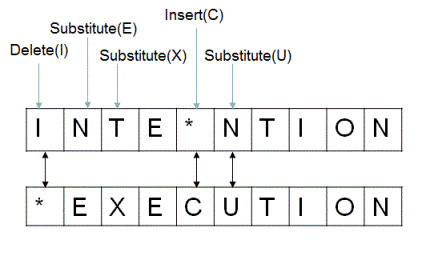
\includegraphics[width=0.7\textwidth]{img/distance.png}
	\end{center}
    \caption{Operácie nad znakmi v slove.}
	\label{fig:levenshtein}
\end{figure}

\subsection{Algoritmus výpočtu Levenshteinovej vzdialenosti}
Základom algoritmu je matica \textit{n + 1} x \textit{m + 1}, pričom \textit{n} je dĺžka prvého slova a \textit{m} je dĺžka druhého slova. S využitím princípu dynamického programovania sa porovnávajú jednotlivé kombinácie prefixov obidvoch slov. Matica má tak naviac jeden riadok a jeden stĺpec, ktoré predstavujú prázdny prefix.

Hlavným problémom je teda určenie minimálnej vzdialenosti - \texttt{D[m,n]}, ktorý je možné rozdeliť na podproblémy tak, že sa určí minimálna vzdialenosť jednotlivých prefixov - \texttt{D[i,j]}, kde \texttt{i} a \texttt{j} sú dĺžky daných prefixov. Matica sa na začiatku inicializuje hodnotami podľa pravidiel \texttt{D[i,0] = i} a \texttt{D[0,j] = 0}. Ďalšie hodnoty sa vypočítajú na základe nasledujúceho vzorca, kde $a_i$ a $b_j$ predstavujú prefixy slov $a$ a $b$:

 \begin{equation}
 \texttt{D[i,j] = min}\begin{cases}
       \texttt{D[i - 1][j - 1] + 1\textsubscript{$a_i \neq b_j$}} \\
       \texttt{D[i][j - 1] + 1} \\
       \texttt{D[i - 1][j] + 1}
       \end{cases}
 \end{equation}

V prvom prípade sa jedná o nahradenie znaku s pripočítaním 1, ak sú znaky na pozíciach $a_i$ a $b_j$ rôzne. Ak nejaké dva prefixy $a_i-1$ a $b_j-1$ majú určitú editačnú vzdialenosť, tak pridaním rôznych znakov k obom prefixom tú vzdialenosť zvýši o hodnotu 1, čo predstavuje práve substitúciu pridaných znakov. Ak sú znaky zhodné, potom substitúcia nie je potrebná, takže vzdialenosť sa nemení. 

V druhom prípade sa jedná o pridanie znaku do prefixu $a_i$ a v treťom prípade sa jedná o odobratie znaku z prefixu $a_i$. Po vypočítaní všetkých hodnôt v matici nám vyjde výsledná hodnota práve na pozícii $[m,n]$.



\chapter{Server}
V tejto kapitole sa zaoberám serverom, ktorý slúži ako backend pre webového klienta a aj pre desktopovú aplikáciu. Pre webového klienta backend poskytuje služby na prácu s dátami, ktoré predstavujú samotné slovníky, a taktiež poskytuje preklad slov z vybraných slovníkov. Pre desktopovú aplikáciu poskytuje služby na synchronizáciu slovníkov.

\section{Použité technológie}
Server je implementovaný v programovacom jazyku Javascript s využitím frameworku Node.js.

\subsection{Node.js}
Technológií pre implementáciu servera je mnoho a ešte pred začiatkom implementácie bolo nutné sa rozhodnúť, ktorú zvoliť. Node.js je pomerne nová technológia, vznikla v roku 2009, avšak odvtedy postupne získavala čoraz viac na popularite.

Hlavnou myšlienkou vzniku bolo využitie Javascriptu aj na strane servera a aj vďaka tomu si Node.js obľúbilo mnoho programátorov, ktorí mali skúsenosti prevažne so skriptovaním na strane klienta práve v tomto jazyku. Ďalšou výhodou bola možnosť využívať aj množstvo javascriptových knižníc, ktoré bolo veľmi jednoduché do aplikácie v Node.js naimportovať. Neskôr však vznikol nástroj na inštalácie externých knižních nazvaný Node Package Manager (NPM).

Základom Node.js je V8 javascriptový interpreter pre Google Chrome. Je založený na asynchrónnom spracovaní udalostí, takže napríklad nevznikajú blokujúce I/O procesy, medzi ktoré patrí prístup k súborom na disku alebo k sieťovým funkciám. Node.js obsahuje rôzne štandardné knižnice, medzi ktoré patrí napríklad File System pre správu súborov alebo HTTP pre správu požiadaviek \parencite{krause2017introduction}.

Node.js je vytvorené pre beh na operačných systémoch Windows, Linux a Mac OS. Výhodou použitia Node.js je jeho jednoduchosť a hodí sa skôr pre menej rozsiahle aplikácie. Práve takáto je však aj táto slovníková aplikácia, ktorá pracuje s malým množstvom dát a nevyžaduje príliš komplexnú funkcionalitu. Z toho dôvodu som si zvolil práve Node.js, ale taktiež aj kvôli mojim skúsenostiam s programovaním v Javascripte.

\subsection{Node Package Manager}
NPM je najznámejší a najpoužívanejší nástroj pre správu javascriptových externých knižníc, či už na strane klienta s využitím rôznych komplexnejších frameworkov, alebo na strane servera využívajúceho Node.js. Pomocou neho sa dajú stiahnuť a zároveň nainštalovať požadované knižnice jednoducho - zadaním príkazu \texttt{npm install} nasledovaného názvom knižnice. Tieto knižnice môže vytvárať ktorýkoľvek programátor alebo programátori, a keď ich oficiálne publikujú, tak si ich môže ktokoľvek nainštalovať a začať používať. Vďaka tomu existuje obrovské množstvo takýchto knižníc.

Konfiguračným súborom je \texttt{package.json}, v ktorom je zoznam použitých knižníc, ktoré sa všetky stiahnu a nainštalujú príkazom \texttt{npm install} a následne je aplikácia pripravená na spustenie. V \texttt{package.json} sa nachádza aj zoznam skriptov, ktoré je potom možné spustiť príkazom \texttt{npm} nasledovaným názvom skriptu.

Knižnice môžu mať tiež svoj vlastný \texttt{package.json}, v ktorom sa nachádza zoznam ďalších knižníc, ktoré samotná knižnica využíva. Pri inštalácii sa vytvorí priečinok \texttt{node\_modules} obsahujúci jednotlivé knižnice a zároveň aj knižnice nainštalované ako ich závislosti.

\subsection{Koa.js}
Koa.js je jeden z frameworkov pre Node.js slúžiaci pre vývoj webových aplikácií. Je to pomerne málo rozsiahla knižnica s jednoduchou funkcionalitou, ale umožňuje rôzne rozšírenia o ďalšie frameworky a to formou funkcií, ktoré fungujú ako middleware. 

V aplikácii sa na začiatku vytvorí objekt obsahujúci metódu \texttt{use}, ktorej parametrom je asynchrónna funkcia - middleware. Tá ma dva vstupné parametre. Prvým z nich je objekt predstavujúci kontext HTTP requestu (\texttt{ctx}) a druhým je asynchrónna funkcia (\texttt{next}), ktorá spúšťa ďalší middleware.

\paragraph{Kontext HTTP requestu}
Kontext obsahuje pod atribútom \texttt{ctx.request} všetky parametre HTTP requestu prijatého na server, napríklad hlavičky, typ HTTP metódy alebo telo requestu. Zároveň je možné nastavovať parametre odpovede, ktorú server bude odosielať, napríklad \texttt{ctx.body} nastaví telo alebo \texttt{ctx.status} nastaví status kód.

\paragraph{Koa middleware}
Na obrázku \ref{fig:koa-middleware} je sekvenčný diagram, v ktorom je znázornené poradie vykonávania jednotlivých middlewarov. To je určené tak, v akom poradí sa zavolajú jednotlivé middleware-y metódou \texttt{use}. Vo funkcii predstavujúcej middleware je možné použiť \texttt{await} pred príkazom 
\texttt{next} a zvyšok príkazov sa tak vykoná až po skončení nasledujúceho middleware-u.


\begin{figure}
	\begin{center}
	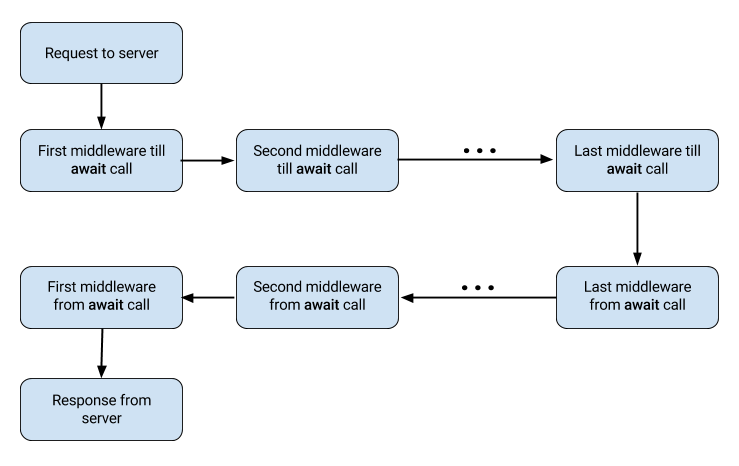
\includegraphics[width=\textwidth]{img/koa-middleware.png}
	\end{center}
    \caption{Koa middleware}
	\label{fig:koa-middleware}
\end{figure}


\section{Architektúra}
Server je implementovaný v programovacom jazyku Javascript s využitím frameworku Node.js. Poskytuje endpointy pre požiadavky na základe protokolu HTTP. V nasledujúcich podkapitolách popisujem základné prvky a návrhové vzory, ktoré server využíva.

\subsection{Aplikačné vrstvy}
Často sa v serverových, ale aj v iných aplikáciach využíva rozdelenie funkcionality na rôzne vrstvy. Môžu to byť konkrétne návrhové vzory, napríklad Facade layer alebo Service layer, z ktorých každá vykonáva špecifickú funkcionalitu. Takéto vrstvy majú komunikovať len so susednými vrstvami. V aplikácii nevyužívam konkrétne návrhové vzory, ale funkcionalita je rozdelená do troch vrstiev.

V najvyššej vrstve sa spracovávajú požiadavky, ktoré prichádzajú na server. Validujú sa parametre HTTP requestov a vytvárajú sa na ne odpovede (HTTP response). Táto vrstva komunikuje s prostrednou volaním jej metód. Má na starosti zavolanie metódy so správnymi argumentami a následné spracovanie výstupu danej metódy, na základe ktorého potom daný HTTP-response tvorí.

Prostredná vrstva predstavuje aplikačnú logiku. Na základe argumentov, ktoré dostane, vykoná špecifickú funkcionalitu. K tej potrebuje samotné dáta, a aby ich získala, využíva poslednú, najnižsiu vrstvu. Príkladom funkcionality môže byť vyhľadávanie slov v slovníkoch. Výsledky potom vracia najvyššej vrstve, prípadne sa môže jednať aj o chybové stavy.

V najnižšej vrstve sa pracuje s dátami, takže obsahuje metódy typu CRUD (create, read, update, delete), ktoré pristupujú priamo k datábaze. Metódy sú teda čo najjednoduchšie a obsahujú funkcionalitu len pre konkrétnu operáciu týkajúcu sa konkrétneho zdroja. Dáta môžu tvoriť slovníky alebo ich uložené zmeny. Táto vrstva tak má nastarosti operácie nad slovami v slovníku, ich ďalšími atribútmi a vytvára zodpovedajúce zmeny pre dané operácie.

\subsection{Client–server model}
Princíp modelu client-server je, že proces, ktorý predstavuje server, spracováva požiadavky prichádzajúce od viacerých klientov. Server potom posiela dáta naspäť klientom, u ktorých sa zobrazujú \parencite{hanson2000client}.

Pri toku dát zo servera ku klientovi sa však zvyčajne vykonáva určitá logika. Tá predstavuje rôzne spracovanie dát - od filtrovania cez usporiadavanie až po formátovanie. Ďalej je potrebné dáta transformovať do formátu HTML, ktorý je určený pre zobrazovanie v internetových prehliadačoch. Pri opačnom toku dát - od klienta na server - je nutné spracovať akcie, ktoré užívatelia vykonávajú.

Táto logika môže byť vykonávaná aj na strane servera a aj na strane klienta a, podľa toho sa aj rozlišujú modely \textit{Thin Client} a \textit{Thick Client}. V prípade modelu \textit{Thin Client} sa väčšina logiky vykonáva na strane servera, v prípade modelu \textit{Thick Client} je veľká časť logiky presunutá na stranu klienta.

Ja som sa snažil väčšiu časť tejto logiky preniesť práve na stranu klienta. Server teda vytvára odpoveď len vo formáte JSON, ktorú následne webový klient spracuje a vytvára zodpovedajúci HTML kód. Užívateľské akcie sú spracovávané na klientovi, ktorý posiela zodpovedajúce požiadavky serveru buď na čítanie, alebo zapisovanie dát.

\subsection{REST API}
Pri vytváraní jednotlivých endpointov som využil princípu architektúry REST (Representational State Transfer). Je to architektúra na jednotný prístup k dátam aplikácie alebo k procedúram s dátami. Každá dátová entita má svoj jedinečný identifikátor označovaný ako URI (Uniform Resource Identifier) \parencite{masse2011rest}. 

Táto architektúra umožňuje pristupovať k zdrojom pomocou metód protokolu HTTP a využíva z nich tieto štyri:
\begin{itemize}
	\item \texttt{GET} na získanie prístupu k dátam
	\item \texttt{POST} na vytvorenie nových dát
	\item \texttt{PUT} na editáciu existujúcich dát
    \item \texttt{DELETE} na vymazanie dát
\end{itemize}

Základnou entitou sú slovníky a všetky služby týkajúce sa práce s nimi začínajú prefixom \texttt{/dictionary}. Služby, súvisiace s prácou s konkrétnym slovníkom, potom majú prefix \texttt{/dictionary/:name}. Ďalej existujú služby na prácu so slovami v slovníku, tie majú prefix \texttt{/dictionary/:name/word}. Podrobný popis služieb sa nachádza v kapitole \ref{sec:api}.

V tejto aplikácii sú všetky odosielané aj prijímané dáta vo formáte JSON, pretože je kompaktnejší, prehľadnejší a najmä je to natívny formát jazyka Javascript, v ktorom je napísaný aj server, aj klient.


\section{Popis služieb API} \label{sec:api}

\texttt{GET api/version}
\begin{itemize}
\item vráti názov a verziu aplikácie a slúži pre desktopového klienta ako overenie, že komunikuje so správnym serverom
\item \begin{lstlisting}[basicstyle=\small]
Response body:
{
  "app":"dictionaryServer",
  "version":"0.1.0"
}
\end{lstlisting}
\end{itemize}

\noindent
\texttt{GET api/dictionary}
\begin{itemize}
\item vráti zoznam všetkých slovníkov s ich základnými parametrami, takže neobsahujú slová s prekladmi
\item slovník obsahuje svoje meno (\texttt{name}), číslo revízie (\texttt{revision}), počet slov (\texttt{wordCount}), dátum vytvorenia (\texttt{createdAt}) a poslendej úpravy slov v slovníku (lastEditedAt)
\item \begin{lstlisting}[basicstyle=\small]
Response body:
[
  {
  	"name": "dictionary1",
  	"revision": 47,
    "wordCount": 42,
    "createdAt": 1495256108553,
    "lastEditedAt": 1495290542671,
  },
  ...
]
\end{lstlisting}
\end{itemize}

\noindent
\texttt{POST api/dictionary}
\begin{itemize}
\item vytvorí nový slovník a vráti číslo jeho revízie
\item parameter \texttt{name} predstavuje meno slovníka a parameter \texttt{text} predstavuje text slov s prekladmi v rovnakom formáte ako v súboroch \texttt{.dict}
\item \begin{lstlisting}[basicstyle=\small]
Request body:
{
  "name": "dictionary1",
  "text": "ein\n one\nzwei\n zwei\ndrei\n three"
}
\end{lstlisting}
\end{itemize}

\noindent
\texttt{GET api/dictionary/:name?json}
\begin{itemize}
\item vráti celý obsah slovníka s menom \texttt{name}
\item ak je prítomný parameter \texttt{json} (napríklad \texttt{json=true}), sú slová vo formáte JSON (\texttt{words}), v opačnom prípade sú v textovom formáte DICT (\texttt{text})
\item \begin{lstlisting}[basicstyle=\small]
Response body (words in JSON):
{
  "name": "string",
  "revision": int,
  ...
  "words": {
  	"word1": "translation1",
    "word2": "translation2",
    ...
  }
}
\end{lstlisting}
\item \begin{lstlisting}[basicstyle=\small]
Response body (words in DICT):
{
  "name": "string",
  ...
  "text": "ein\n one\nzwei\n zwei\ndrei\n three..."
}
\end{lstlisting}
\end{itemize}

\noindent
\texttt{DELETE api/dictionary/:name}
\begin{itemize}
\item vymaže slovník s menom \texttt{name} zo servera
\end{itemize}

\noindent
\texttt{POST api/dictionary/:name/word/}
\begin{itemize}
\item vytvorý v slovníku nové slovo s novým prekladom, ak sa slovo na serveri ešte nevyskytuje, inak priradí preklad k už existujúcemu slovu 
\item \begin{lstlisting}[basicstyle=\small]
Response body:
{
  "word": "ein",
  "translation": "jedna"
}
\end{lstlisting}
\end{itemize}

\noindent
\texttt{PUT api/dictionary/:name/word/}
\begin{itemize}
\item zmení slovo v parametri \texttt{word} na nové slovo \texttt{newWord} s novým prekladom \texttt{newTranslation}
\item ak nie je prítomný parameter \texttt{newWord}, tak slovo ostáva nezmenené a zmení sa len jeho preklad
\item \begin{lstlisting}[basicstyle=\small]
Response body:
{
  "word": "ein",
  "newWord": ""
  "newTranslation": "jedna"
}
\end{lstlisting}
\end{itemize}

\noindent
\texttt{DELETE api/dictionary/:name/word/:word}
\begin{itemize}
\item vymaže slovo \texttt{word} zo slovníka s menom \texttt{name}
\end{itemize}

\noindent
\texttt{POST api/sync/dictionary/:name}
\begin{itemize}
\item slúži pre synchronizáciu slovníka desktopového klienta so slovníkom na serveri
\item server dostáva zmeny z desktopového klienta a zároveň mu posiela vlastné zmeny
\item \begin{lstlisting}[basicstyle=\small]
Request body:
{
  "revision": 5,
  "changes": [
    {
      "type": "add",
      "word": "word1",
      "translation": "translation1"
    },
    ...
  ]
}
\end{lstlisting}
\item \begin{lstlisting}[basicstyle=\small]
Response body:
{
  "revision": 5,
  "changes": [
    {
      "type": "add",
      "word": "word1",
      "translation": "translation1"
    },
    ...
  ]
}
\end{lstlisting}
\end{itemize}

\noindent
\texttt{GET api/translate?word\&dict}
\begin{itemize}
\item vráti zoznam prekladov k danému slovu z parametra \texttt{word}, ktoré hľadá v slovníkoch uvedených vo viacnásobných parametroch \texttt{dict}
\item parameter \texttt{word} môže byť reťazec viacerých slov, ktoré sa následne rozpársujú na jednotlivé slová pre vyhľadávanie prekladov
\item ak nie je prítomný žiadny parameter \texttt{dict}, preklady sa vyhľadávajú vo všetkých dostupných slovníkoch
\item preklad obsahuje vyhľadávané slovo \texttt{key}, slovo (\texttt{word}), ktoré sa našlo v slovníku, jeho preklad (\texttt{translation}), Levenshteinovu vzdialenosť (\texttt{distance}) medzi vyhľadávaným a nájdeným slovom, a slovník (\texttt{dict}), v ktorom bolo slovo nájdené
\item \begin{lstlisting}[basicstyle=\small]
Response body:
[
  {
    "word": "word1",
    "key": "word",
    "translation": "translation1",
    "distance": 1,
    "dict": "dictionary1"
  },
  {
    "word": "word2",
    "key": "word",
    "translation": "translation2",
    "distance": 1,
    "dict": "dictionary2"
  },
  ...
]
\end{lstlisting}
\end{itemize}


\section{Ukladanie dát}
V desktopovej aplikácii sú slovníky uložené v textových súboroch vo formáte \texttt{.dict}. Každé slovo je na samostatnom riadku a k nemu priradený preklad je na novom riadku pod daným slovom a začína medzerou. Preklad môže tvoriť aj viacero slov, tie sú všetky na jednom riadku oddelené znakom \texttt{;}. Slovník sa do desktopovej aplikácie načíta zo súboru a je uložený v pamäti ako reťazec (\texttt{std::string}).

\theoremstyle{definition}
\newtheorem{exmp}{Príklad}[chapter]
\begin{exmp}
Formát slovníku
\centering
\begin{lstlisting}[basicstyle=\small]
sprechen
 speak; talk
reisen
 travel
einmal
 once; one day
\end{lstlisting}
\end{exmp}

Na uloženie slovníka však existuje viacero možností. Medzi klasickú voľbu pri implementácii serverových aplikácií patrí napríklad SQL, prípadne NoSQL databáza. Databáza je ale vhodná na ukladanie komplexnejších entít, a v prípade slovníku sa jedná o jednoduchú entitu. Navyše pri dotazovaní sa na dáta kvôli prekladu je vždy potrebný celý slovník, preto je vhodné ho mať stále v pamäti. Serverová aplikácia tak používa in-memory databázu na prácu s dátami a na permanentné uloženie využíva súbory.

\subsection{In-memory databáza} \label{sec:inmemorydb}
Server má v pamäti uložené slovníky každý ako jeden objekt, ktorý funguje ako hash mapa. V Javascripte, konkrétne v engine V8, je implementovaný objekt ako pole, v ktorom sú kľúče objektu pomocou nejakej hashovacej funkcie mapované na indexy poľa. Prístup na takýto prvok cez kľúč je konštantný. Slová slovníka je možné uložiť ako pár kľúč-hodnota, pričom kľúčom je samotné slovo a hodnotu predstavuje jeho preklad.

\begin{exmp}
Štruktúra slov slovníku v pamäti
\centering
\begin{lstlisting}[basicstyle=\small]
{
  "sprechen": "speak; talk",
  "reisen": "travel",
  "einmal": "once; one day"
}
\end{lstlisting}
\end{exmp}

\subsection{String vs. Hash map}
Pre porovnanie dátovej štruktúry reťazca a hash mapy boli vytvorené testy, v ktorých sa vyhľadávala skupina slov v jednotlivých štruktúrach a pri vyhľadávaní sa vypočítavala Levenshteinova vzdialenosť. Testovacie dáta predstavoval slovník s počtom slov 81472. V ňom boli vyhľadávané štyri slová, konkrétne \textit{schwimmen, willkommen, katze} a \textit{grose}. Pre obe štruktúry boli zmerané počty milisekúnd, ktoré predstavujú časovú zložitosť prehľadávania danej štruktúry.

Prehľadávanie hash mapy si vyžaduje iteráciu cez jednotlivé kľúče, prehľadávanie reťazca si vyžaduje iteráciu cez jednotlivé znaky v reťazci. Tých je síce oveľa viac ako kľúčov, ale pri hash mape je nutné ich mapovanie na položky v poli. Výsledkom je teda mierne efektívnejšie prehľadávanie práve v hash mape, ako znázorňuje tabuľka \ref{tab:string-hash}.

Ďalším zaujímavým parametrom je využitie operačnej pamäte. Hash mapa jej využíva podstatne viac ako reťazec, kedže potrebuje mať popri samotných slovách a prekladoch uložených aj množstvo referencií a ďalších atribútov. V tabuľke sú dáta po načítaní rovnakého slovníka ako v tom, ktorý bol použitý pri testovaní vyhľadávania.

Dôvodom pre použitie hash mapy miesto reťazca bol konštantný prístup k jednotlivým slovám. V reťazci by bolo potrebné vždy prechádzať slovník, aby bolo možné slovo nájsť. Takýto prístup ku konkrétnemu slovu je nutný pri operáciách so slovami, akými sú pridanie, editácia a zmazanie slova. Ďalším dôvodom bolo to, že hash mapa už má slová a ich preklady rozpársované a tak sa jednoduchšie pracuje s takouto štruktúrou, ako s celým reťazcom. 

\begin{table}[]
\centering
\caption{String vs. Hash map}
\label{tab:string-hash}
\begin{tabular}{lll}
     & Hash map & String   \\
Time & 640 ms   & 820 ms   \\
Memory used & 23 773 kB & 12 027 kB
\end{tabular}
\end{table}

\subsection{JSON súbor}
Každý slovník je uložený v samostatnom súbore vo formáte JSON. Pre Javascript je to prirodzený formát a je jednoduché takéto súbory pársovať do objektu, pretože je to natívna funkcionalita metódy \texttt{require}, ktorá slúži na importovanie Javascriptových súborov a modulov. Navyše formát JSON presne popisuje štruktúru objektov v Javascripte.


\section{Implementácia}
\subsection{Asynchrónne metódy}
V prvotných verziách Node.js boli udalosti, ktoré sa volali po skončení asynchrónnej metódy, implementované pomocou funkcií (zvaných callback), ktoré boli predané ako parametre do danej metódy. S príchodom ECMA Scriptu 2015 sa začali tieto funkcie nahrádzať Promisami. Tie už neboli parametrom asynchrónnej metódy, ale jej výstupnou hodnotou. Promisa obsahuje metódu \texttt{then}, ktorej parametrom je callback po úspešnom skončení Promisy, a ďalej metódu \texttt{catch}, ktorej parametrom je callback pre chybový stav v Promise.

ECMA Script 2016 priniesol do Javascriptu kľúčové slová \texttt{async} a \texttt{await}, ktoré sú podporované v Node.js od verzie 7.6, a sú použité v implementácii servera slovníkovej aplikácie. Stále sa využívajú Promisy a \texttt{await} je iba syntakticky inak napísaný \texttt{then}, avšak prináša prehľadnejšiu štruktúru kódu.

Úplne prvou asynchrónnou metódou po spustení programu je práve spustenie servera. Na to slúži metóda \texttt{listen} z frameworku Koa. Pri spracovaní HTTP requestov sa tieto metódy využívajú, čo znamená, že sa dve rôzne požiadavky môžu spracovávať paralélne. Výhodou toho je, že na začatie spracovávania jednej požiadavky nie je potrebné, aby sa spracovávanie druhej pred tým ukončilo.

\subsection{Routing}
Pre identifikáciu API služieb bol použitý modul \texttt{koa-router}, ktorý funguje ako middleware pre modul \texttt{koa}. Každé spracovanie API služby funguje ako samostatný middleware. Každý middleware porovnáva URL a HTTP metódu a podľa nich buď začne vykonávať kód určený pre danú službu, alebo len zavolá ďalší middleware v poradí.

Na začiatku sa vytvorí objekt \texttt{router}, ktorý obsahuje metódy s názvami zhodnými s názvami klasických HTTP metód. Tie majú ako prvý parameter URL, podľa ktorého je spolu s názvom danej metódy možná identifikácia konkrétnej služby. Spracovanie napríklad služby \texttt{GET api/dictionary/:name} môže vyzerať nasledovne:

\begin{exmp}
Spracovanie HTTP požiadavku
\centering
\begin{lstlisting}[basicstyle=\small]
router.get('/dictionary/:name', async (ctx, next) => {
  const name = ctx.params.name
  const dict = DictController.findDictionary(name)
  
  ctx.body = dict
})
\end{lstlisting}
\end{exmp}

Ak je prefix \texttt{api/} nastavený v počiatočnej konfigurácii routra, tak sú všetky služby spracovávané spolu s týmto prefixom. Nie je teda potrebné ho písať do URL v každej metóde. Výhodou je aj možnosť tento prefix zmeniť kedykoľvek pre všetky metódy naraz.

Koa-router má aj klasickú metódu \texttt{use}, ktorá funguje rovnako ako \texttt{use} priamo v Koa, takže je možné pridávať middleware-y takým istým spôsobom.

\subsection{Validácia HTTP requestov}
Pri HTTP requeste je možné validovať viacero druhov parametrov. REST API server využíva parametre URL pre identifikáciu zdrojov, ďalej využíva parametre z \textit{query} časti URL a využíva aj telo requestov - \textit{Request body}. Na ich validáciu je použitá knižnica Koa-validate, ktorá rozširuje framework Koa. Konkrétne pridáva priamo do objektu \textit{ctx} validačné metódy, ktoré potom vytvoria aj relevantnú HTTP odpoveď v podobe chybových hlášok o vyskytnutých chybách (\texttt{ctx.errors}).

Pre identifikáciu konkrétneho parametra sa používajú tri základné metódy. Konkrétne \texttt{checkParams("url-param")} pre identifikáciu základných parametrov URL, \texttt{checkQuery("queryParam")} pre identifikáciu \textit{query} časti URL a \texttt{checkBody("bodyParam")} pre identifikáciu parametrov \textit{Request body}.

Na spomenuté metódy je potom možné reťaziť validačné metódy, ktoré validujú daný parameter. Umožňujú validovať typ parametra (\texttt{isInt()}), či je prítomný, respektíve či nie je prázdny (\texttt{notEmpty()}), a umožňujú validovať nejaké jeho vlastnosti, napríklad pomocou regulárneho výrazu (\texttt{match()}, prípadne \texttt{notMatch()}).

Validácia \texttt{notEmpty()} sa využíva hlavne v requestoch typu POST a PUT pre zistenie, či sú prítomné povinné dáta pre vytvorenie, prípadne editáciu. Napríklad pri vytvorení alebo editácii slova musí byť prítomné vždy dané slovo a aj jeho preklad. 

Pri názvoch slovníkov existuje obmedzenie na niektoré znaky kvôli tomu, že daný názov sa používa aj pre názov príslušných súborov, ktoré by tak nebolo možné vytvoriť v závislosti od používaného operačného systému. Pri zjednotení týchto znakov dostávame množinu znakov $\slash < > * ? \backslash \% : . "  \vert$

Pri konkrétnych slovách je tiež obmedzenie na špecifické znaky, pretože slovo by malo pozostávať hlavne z písmen, a navyše pri prístupe k týmto slovám v Lowdb pomocou metód \texttt{get} a \texttt{set} by niektoré znaky mohli byť brané ako kľúčové znaky pre prístup k ďalším atribútom objektu. Všetky bežne používané interpunkčné znamienka sú pri spracovaní slova brané ako rozdelenie tohto slova v mieste výskytu znamienka na dve, prípadne viac slov, ak je znamienok v slove viac. Výnimkou sú znaky apostrof a pomlčka, ktoré sú do slova akceptované, pretože môžu byť súčasťou niektorých slov. 

\subsection{Error handling}
Chybové stavy servera môžu predstavovať chyby, ktoré vznikli buď na základe očakávaných, alebo neočakávaných akcií v behu programu. Medzi tie očakávané patria tie, ktoré vyplývajú s nesprávneho HTTP requestu. Tými sú:
\begin{itemize}
\item dotaz na neexistujúci slovník
\item dotaz na vyvorenie alebo synchronizáciu slovníka s menom, ktoré už nejaký iný používa
\item dotaz na neexistujúce slovo v slovníku
\item nesprávny formát požiadaviek - chýbajúce parametre, nevalidné parametre a iné
\end{itemize}

Tieto chybné požiadavky sú ošetrené a vytvárajú sa na ne odpovede s relevantným status kódom a chybovou hláškou. Na príklade \ref{exmp:error} je odpoveď servera na dotaz na neexistujúci slovník. Neočakávané chyby sú zachytené middlewarom, ktorý je použitý ako prvý v poradí metódou \texttt{use} z Koa, takže pokrýva všetku ďalšiu logiku spracovania požiadavky.

\begin{exmp}
\label{exmp:error}
Odpoveď servera o chybovom stave
\centering
\begin{lstlisting}[basicstyle=\small]
HTTP request: GET api/dictionary/German%20Dictionary

HTTP response:
{
  "error": "Dictionary 'German Dictionary' not found.",
  "code": 400
}
\end{lstlisting}
\end{exmp}

\subsection{Databáza}
Uloženie dát je rozdelené do dvoch sekcií - operačná pamäť a súbory typu JSON, ktoré má daný slovník dva - jeden pre ukladanie slov a druhý pre ukladanie zmien nad týmito slovami. Pri zmene dát v slovníku je nutné uložiť túto zmenu aj do príslušných súborov, na to je použitá Javascriptová knižnica Lowdb. Je to veľmi jednoduchá knižnica, ktorá funguje ako súborová databáza určená na prácu so súbormi typu JSON, ale podporuje aj ďalšie formáty, napríklad BSON alebo XML.

Lowdb umožňuje ukladanie dát do klasického javascriptového objektu (spomínana hash mapa z kapitoly \ref{sec:inmemorydb}. Pri spustení aplikácie je vytvorený objekt zavolaním \texttt{lowdb('path/to/file.json)} s parametrom cesty k danému súboru. V zložke \texttt{dictionaries} sa nachádzajú súbory s názvom slovníku a v zložke \texttt{meta} sa nachádzajú súbory pre ukladanie zmien s názvom slovníku doplneným prefixom \texttt{\_} (napr. \_dictName.json). Pre každý súbor je tak vytvorený samostatný Lowdb objekt.

Ten obsahuje metódy na prístup k atribútom objektu, napríklad \texttt{get()} na získanie hodnoty a \texttt{set()} na zapísanie hodnoty. Parametrom obidvoch metód je názov atribútu, ktorý predstavuje kľúč v hash mape, a metóda \texttt{set} má ako parameter navyše ešte hodnotu, ktorú zapisuje.

Lowdb poskytuje okrem metód \texttt{get} a \texttt{set} aj množstvo ďalších a to konkrétne metódy z knižnice Lodash. Tá obsahuje metódy pre prácu s javascriptovými kolekciami, ktoré sa dajú rovnako použiť pre dáta v Lowdb. Ďalšou dôležitou metódou je \texttt{write()}, ktorá vykonané zmeny uloží do súboru.

\subsection{Parsovanie}
Pri prekladaní slova pomocou služby \texttt{GET api/translate?word\&dict} sa v parametri \texttt{word} nachádza reťazec, ktorý môže obsahovať viacero slov. Tie sa parsujú z reťazca jednak podľa medzier, ktorými sú oddelené, a navyše aj podľa špecifických znakov alebo vlastností určených na rozdelenie slov.

Na vyhľadanie týchto znakov sú použité regulárne výrazy a medzi potenciálne slová sa vloží medzera. Takéto rozdelenie umožňuje pomocou javascriptovej funkcie \texttt{String.prototype.split(' ')} vytvoriť pole slov, s ktorým je už jednoduché pracovať. Regulárne výrazy pre predpokladané programátorské menné konvencie sú nasledovné:
\\

\noindent
\texttt{/C[A-Z][a-z]+/g}
\begin{itemize}
\item Táto menná konvencia predpokladá výskyt veľkého písmena \textit{C} pred nejakým slovom začínajúcim tiež veľkým písmenom a znamená označenie triedy (Class).
\item Príkladom z reťazca \texttt{CKreis} chceme dostať slovo \texttt{kreis}.
\end{itemize}

\noindent
\texttt{/[a-z][A-Z]/g}
\begin{itemize}
\item Určené pre parsovanie v prípade konvencie s názvom Camel case
\item Príkladom z reťazca \texttt{findeLetztenIndex} chceme dostať slová \texttt{finde}, \texttt{letzten} a \texttt{index}.
\end{itemize}

\noindent
\texttt{/[A-Z]{2,}/g}
\begin{itemize}
\item Detekcia konvencie Upper case, pri ktorej všetky písmená v slove sú veľké.
\item Príkladom z reťazca \texttt{undSCHNELL} chceme dostať slová \texttt{und} a \texttt{schnell}.
\end{itemize}

\noindent
\texttt{/\_/g}
\begin{itemize}
\item Detekcia konvencie Snake case, podľa ktorej sú slová oddelené znakom \_ (podtŕžnik).
\item Príkladom z reťazca \texttt{FILTER\_LEERE\_ELEMENTE} chceme dostať slová \texttt{filter}, \texttt{leere} a \texttt{elemente}.
\end{itemize}

Dôležité je aj poradie, v ktorých sa dané regulárne výrazy aplikujú. Napríklad parsovanie slov s prefixom \textit{C} prebieha ešte pred Upper case parsovaním, pretože potom by sa napríklad slovo \texttt{CKreis} rozdelilo na slová \texttt{CK} a \texttt{reis}.

Príkladom jedného vyhľadávania môže byť nasledovný reťazec: \texttt{CLesenFlauming\_falshGeshrieben word einfachUndSCHNELL}, ktorý sa rozparsuje na slová \texttt{lesen}, \texttt{flaumig}, \texttt{falsh}, \texttt{geschrieben}, \texttt{worte}, \texttt{einfach}, \texttt{und} a \texttt{schnell}. Pri jednom prekladaní sa tak všetky tieto slová vyhľadávajú zvlášť.

\subsection{Práca so slovníkom}
Prvým krokom v práci s nejakým slovníkom je jeho vytvorenie. To spočíva vo vytvorení dvoch súborov pomocou funkcie z Lowdb, ktorá zároveň vytvorí príslušné objekty v pamäti. Vytvorenie slovníku môže znamenať aj počiatočnú inicializáciu slov z prijatého textu, ktorý sa parsuje na základe formátu DICT.

Ďalšími funkciami pre prácu so slovníkom, konkrétne s jeho slovami, sú \texttt{addWord()} pre pridanie slova, \texttt{changeWord()} pre editáciu slova a \texttt{deleteWord()} pre jeho zmazanie. Tieto metódy sa vyskytujú vo vrstve aplikačnej logiky, aj v databázovej vrstve.

Pri metóde \texttt{addWord()} sa kontroluje, či dané slovo v slovníku už náhodou neexistuje, pretože ak áno, toto slovo sa nemôže vytvoriť. Neumožňuje to základný princíp hash mapy, ktorá môže obsahovať vždy maximálne jeden unikátny kľúč. V takom prípade sa preklad daného slova uloží k už existujúcemu slovu a rozšíri tak jeho preklad.

Pri rozšírení prekladu sa rozparsujú jednotlivé slová pôvodného aj nového prekladu podľa znaku bodkočiarka (;) a tie sa následne zlúčia do jedného reťazca, ale s vynechaním duplicít. Využité sú funkcie \texttt{String.prototype.split(';')} na vytvorenie poľa slov, z ktorého sa odstraňujú duplicity, a \texttt{Array.prototype.join('; ')} na zlúčenie slov naspäť do reťazca.

Takýto istý prípad môže nastať aj pri metóde \texttt{changeWord()}, ak sa zmení samotné slovo na nejaké nové, ktoré už slovník obsahuje. Vtedy sa preklady zlučujú rovnako. Metóda má nepovinný parameter \texttt{newWord}, ktorý, ak je prítomný, predstavuje zmenu slova, a ak prítomný nie je, mení sa iba jeho preklad.

Na datábazovej vrstve sa využívaju Lowdb funkcie \texttt{set("key", "value")} a \texttt{unset("key")}. \texttt{Set} nastavuje slovu ("key") jeho preklad ("value") a \texttt{unset} vymaže slovo ("key") zo slovníka. Pridanie slova sa tak uskutočňuje zavolaním \texttt{set("word", "translation")}, ktoré využíva aj zmena slova, kedže \texttt{set} pôvodnú hodnotu prepíše novou hodnotou. Ak zmena slova zahŕňa aj zmenu na \texttt{newWord}, tak sa zavolá metóda \texttt{unset("word")}, kde parameter "word" predstavuje pôvodné slovo. Táto metóda sa rovnako volá aj pri vymazaní slova.

\subsection{Ďalšie použité knižnice}
Z knižnice Lodash využívam viacere funckie pre prácu s Javascriptovými dátovými štruktúrami a zároveň ju používa knižnica Lowdb. Lodash obsahuje klasické metódy, ktoré sú aj súčasťou natívneho jazyka Javascript, a mnohé ďalšie, ktoré uľahčujú programátorom prácu. Navyše obsahujú aj validáciu vstupov a optimalizáciu funkctionality.

Z frameworkov, ktoré doplňujú Koa.js pomocou middlewarov, stojí za zmienku Koa-body. Ten parsuje telo HTTP requestov do objektu vo formáte JSON a zároveň dekóduje špeciálne znaky z URL. Pri vývoji aplikácie bol užitočný modul Nodemon, ktorý sledoval zmeny v súboroch so zdrojovým kódom a reštartoval automaticky server, takže som to nemusel robiť ja ručne. 


\section{Synchronizácia slovníkov}
Úlohou servera je poskytovať cloudové úložisko dát, ktoré by mali byť dostupné pre desktopové aplikácie pre synchronizovanie jednotlivých slovníkov. Desktopový klient môže upravovať svoje dáta aj v offline režime a tieto zmeny si postupne ukladá. Klientov môže byť viacero a každý môže mať rôzne zmeny v svojich dátach. Synchronizáciou sa tak má umožniť, aby všetky sa zmeny od rozličných klientov ukladali na jedno miesto - server a mohli sa tak vykonané zmeny zdieľať medzi všetkými klientmi.

Pri synchronizácií slovníkov je požadovaným výstupným stavom ten, pri ktorom majú slovníky v rôznych klientoch rovnaké dáta. Ideálnym stavom je taktiež, ak sa čo najviac dát zachová, ale to nie je možné vždy dosiahnuť, kedže v zmenách môžu nastať konflikty. Dáta, ktoré sa nijakým spôsobom nemenili, musia zostať taktiež zachované.

\subsection{Postup syncrhonizácie}
Iniciátorom synchronizácie je desktopový klient, ktorý je online . Kroky synchronizácie sú znázornené na obrázku \ref{fig:synchronisation}. Po overení dostupnosti servera si z neho stiahne zoznam všetkých slovníkov, ktoré na ňom aktuálne sú. Svoje slovníky potom začne synchronizovať s využitím služny \texttt{POST api/sync/dictionary/:name}. Ak klient vytvoril nejaký nový slovník, keď bol v offline režime, a tento slovník má označený ako synchronizovateľný, tak sa slovník na serveri vytvorí tiež, ale cez službu \texttt{POST api/dictionary}

Pre každý slovník, ktorý je na serveri, klient posiela svoje zmeny spolu s revíziou slovníka, ktorú má uloženú od poslednej synchronizácie. Služba synchronizuje vždy práve jeden slovník, ktorý je daný parametrom \texttt{name}. Server prijaté zmeny spracuje a zároveň posiela klientovi svoje zmeny, ktoré ešte klient podľa revízie slovníka nemá. V HTTP requeste sa teda nachádzajú zmeny klienta a v odpovedi naň sa nachádzajú zmeny servera.

Ak klient aktivuje nový slovník, ktorý predtým nemal, tak sa následne stiahne cez službu \texttt{GET api/dictionary/:name}. Klient môže mať stiahnuté všetky slovníky, ktoré sú na serveri a to v rovnakom stave. Server má všetky slovníky klienta okrem tých, ktoré má klient označené ako nesynchronizovateľné.

\begin{figure}
	\begin{center}
	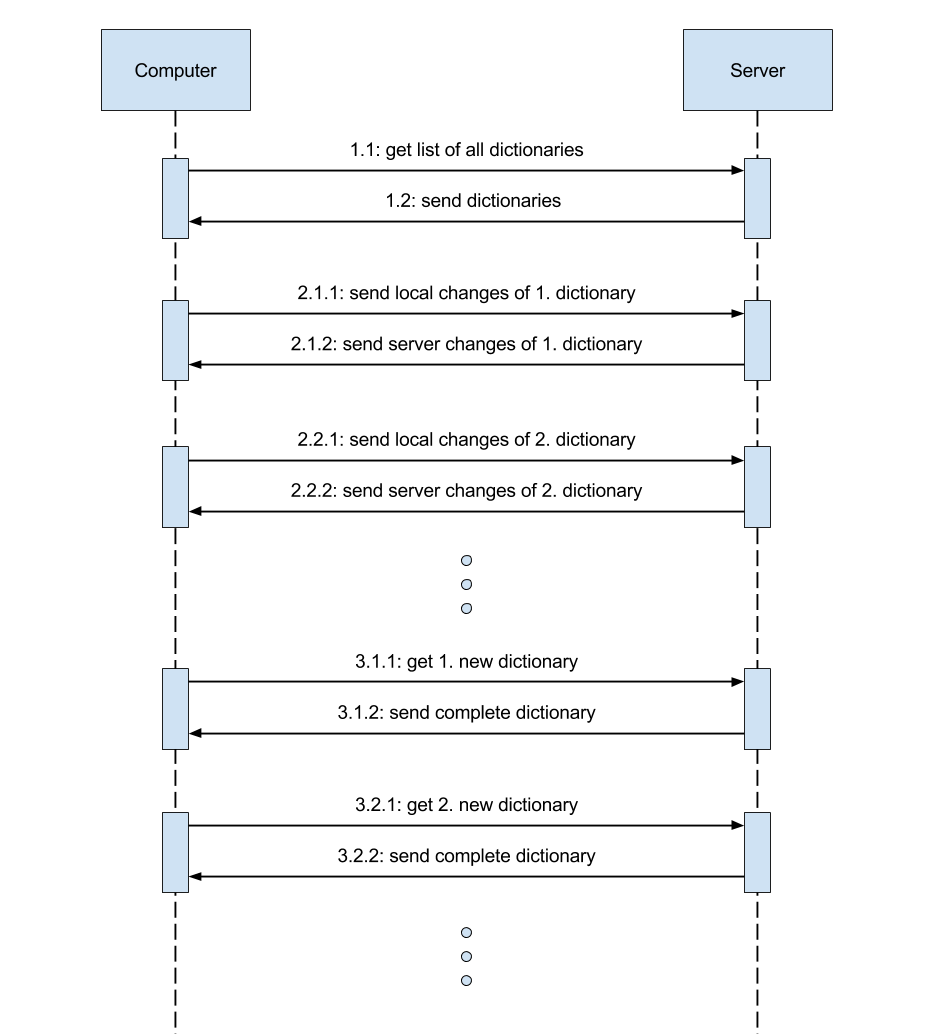
\includegraphics[width=\textwidth]{img/synchronisation.png}
	\end{center}
    \caption{Sekvenčný diagram synchronizácie}
	\label{fig:synchronisation}
\end{figure}

\subsection{Revízia slovníku}
Revízia je číslo, ktoré určuje aktuálnosť daného slovníka a slúži na identifikáciu nových zmien pre server. Počiatočná revízia pri vytvorení slovníka na serveri je 1 a pri pridávaní nových zmien sa postupne zvyšuje s každou zmenou o hodnotu 1. Pri synchronizácii sa aktuálna revízia posiela klientovi, ktorý si danú hodnotu udržuje až po ďalšiu synchronizáciu. Čím väčší je teda rozdiel medzi revíziami servera aj klienta, tak tým viac zmien klientovi chýba a tým viac je jeho verzia slovníku staršia.

Pri synchronizácii sa na serveri nájdu všetky zmeny, ktoré majú vyššiu hodnotu svojej revízie ako revízia klienta. Tieto zmeny sú nové a môžu pochádzať buď od jedného alebo aj viacerych desktopových klientov, ale aj od webových klientov. Všetky ich je však potrebné poslať klientovi, ktorý si slovník synchronizuje.

Server si ukladá len určitý počet zmien a tak sa môže stať, že nejaký klient má staršiu revíziu, ako je najstaršia revízia uložená na serveri. Vtedy je potrebné poslať klientovi celý obsah slovníku miesto zmien.

\subsection{Ukladanie zmien}
Zmeny sa ukladajú vo forme operácií nad slovami v slovníkoch, ktorými sú \textit{addWord}, \textit{changeWord} a \textit{deleteWord}. S každou operáciou sa uloží do súboru objekt reprezentujúci zmenu vo formáte JSON a pridá sa tak na koniec pola zmien. Jeho štruktúru tvoria atribúty \texttt{revision} a \texttt{changes}, ako môžeme vidieť na príklade \ref{exmp:metafile}. Každej jednej zmene je tak priradená revízia, ktorá sa s každou ďalšou zmenou zvyšuje.

\begin{exmp}
\label{exmp:metafile}
Štruktúra zmien slovníku
\centering
\begin{lstlisting}[basicstyle=\small]
"revisions": [
  {
    "revision": 1,
    "changes": null
  },
  {
    "revision": 2,
    "changes": {
      "type": "add",
      "word": "ein",
      "translation": "one"
    }
  },
  {
    "revision": 3,
    "changes": {
      "type": "delete",
      "word": "ein"
    }
  },
  ...
]
\end{lstlisting}
\end{exmp}

Atribút \texttt{type} objektu \texttt{changes} označuje typ zmeny, ale na rozdiel od troch typov operácií nad slovníkom existujú iba dva typy zmien - \texttt{add} a \texttt{delete}. Typ \texttt{add} predstavuje operáciu \textit{addWord}, typ \texttt{delete} predstavuje operáciu \textit{deleteWord} a operácia \textit{changeWord} je reprezentovaná dvoma zmenami ako typ \texttt{delete} nasledovaný typom \texttt{add}.

Počiatočná konfigurácia súboru zmien pri vytvorení slovníku je pole s objektom s atribútmi \texttt{"revision": 1} a \texttt{"changes": null}. Pri vytvorení slovníku v desktopovej aplikácii je počiatočná revízia nulová, takže je možné podľa toho zistiť, že daný slovník ešte nebol synchronizovaný so serverom ani raz. To zabraňuje synchronizácii dvoch rôznych slovníkov s rovnakým názvom.

\subsection{Spracovanie zmien}
Spracovanie je proces na serveri, pri ktorom sa aplikujú prijaté zmeny na daný slovník a zároveň sa vyhľadajú zmeny, ktoré treba poslať klientovi. Server prijaté zmeny prechádza a podľa typu operácie volá metódy \textit{addWord} a \textit{deleteWord} rovnako, ako keby dostal HTTP-request na služby pre pridanie alebo zmazanie slova.

Odoslané zmeny klient aplikuje rovnakým spôsobom, ale ak sa nejaká z prijatých týka rovnakého slova ako nejaká z odosielaných, tak by mohol byt porušený základný princíp synchronizácie, ktorým je konzistentnosť slovníkov. Príkladom môže byť zmena prekladu slova \textit{wort}, ktorá prišla od klienta, a zmazanie slova \textit{wort}, ktoré je na serveri. Po aplikácii zmien by tak na serveri malo byť slovo \textit{wort} a na klientovi by byť nemalo.

Prijaté zmeny je potrebné aplikovať tak, aby konečný stav slovníka odpovedal stavu slovníka na klientovi po odoslaní zmien. Preto je potrebné vyriešiť potenciálne konflikty, ktoré môžu nastať pri rôznych zmenách na rovnakom slove. Rozdelenie operácie \textit{changeWord} na zmeny typu \texttt{add} a \texttt{delete} tento problém značne uľahčuje, pretože je tak jednoduchšie identifikovať zmeny pre konkrétne slovo, keďže \textit{changeWord} sa môže týkať až dvoch slov, pokiaľ sa nemení len preklad, ale aj slovo na nejaké iné.

Ďalšou výhodou ukladania zmien len do dvoch typov je jednoznačnosť výskytu slov. Podľa typu sa dá určiť, či sa slovo v slovníku vyskytuje alebo nie, stačí sa pozrieť na jeho poslednú zmenu. Jednotlivé zmeny je tak možné zredukovať v prípade, že určité slovo bolo zmenené viackrát za sebou a niektoré jeho uložené zmeny sa tak môžu opakovať alebo ich nie je potrebné na slovník aplikovať, pretože nejaké nasledujúce zmeny určia konečný stav slova bez ohľadu na predchádzajúce zmeny.

\subsection{Redukcia zmien}
Zmeny si vieme rozdeliť podľa konkrétnych slov, ktorých sa týkajú a pre každé slovo, vieme odstrániť jeho nepotrebné zmeny. Príkladom môže byť viacnásobné použitie operácie \textit{changeWord} na zmenu prekladu slova, pričom stačí aplikovať iba posledný výskyt tejto operácie, keďže slovo vždy vymaže a vytvorí nové spolu s novým prekladom a preklady vytvorené predtým už slovo obsahovať nebude.

Zmeny jedného slova si môžeme rozdeliť na tri prípady podľa ich postupnosti:
\begin{itemize}
\item $\texttt{add}_1$, $\texttt{add}_2$, ..., $\texttt{add}_n$ - postupnosť operácií zložená výhradne z typov \texttt{add}
\item ..., $\texttt{delete}_{m}$, $\texttt{add}_{m+1}$, ..., $\texttt{add}_n$ - postupnosť obsahujúca aspoň jednu operáciu \texttt{delete} nasledovanú aspoň jednou operáciou \texttt{add}
\item ..., $\texttt{delete}_{n}$ - postupnosť, ktorej posledná operácia je \texttt{delete}
\end{itemize}

V prvom prípade sa jedná o pridanie slova, ktoré môže byť viacnásobné, takže pribúdajú nové preklady. Ak slovník slovo už obsahoval, všetky pôvodné preklady sa zachovávajú. V prípade výskytu \texttt{delete} a ukončením postupnosti operáciou \texttt{add} sa pôvodné preklady slova nezachovajú a vzniknú nové. Konkrétne sú to len tie, ktoré sa nachádzajú za poslednou operáciou \texttt{delete}, pretože všetky, ktoré boli pred ňou, budú tiež vymazané. V prípade, keď je \texttt{delete} poslednou operáciou v postupnosti, sa taktiež nezachovajú žiadne preklady a ani žiadne nepribudnú, pretože slovo sa zo slovníka vymaže úplne.

Odstránením všetkých zmien pred posledným výskytom zmeny \texttt{delete} sa zmeny dajú zredukovať. Nevadí ani, ak sa odstránia zmeny typu \texttt{delete}, kedže poslednou zmenou \texttt{delete} sa slovo maže tak či tak. Vo výsledku redukcie zmien sa tak vyskytuje nejaká zmena \texttt{delete} buď práve jedenkrát, ak v pôvodnej postupnosti bola aspoň jedna taká zmena, alebo ani raz, ak nebola.

\subsection{Zlúčenie konfliktných zmien}
Pri zlučovaní konfliktných zmien (týkajúcich sa rovnakého slova) musí vzniknúť konzistentný stav slovníkov po aplikácii zlúčených zmien. To v niektorých prípadoch môže znamenať, že je potrebné z prijatých alebo odosielaných zmien odstrániť alebo naopak im pridať nejaké ďalšie zmeny pre dosiahnutie konzistencie.

V prvom kroku sa rozdelia zmeny do samostatných postupností podľa toho, ktorému slovu prislúchajú. Slová z prijatých zmien sa potom porovnajú so slovami z odoslaných zmien. Pri zmenách rôznych slov nie je potrebné riešiť konflikty, takže tie sa zachovávajú v nezmenenom stave. Pri zmenách rovnakých slov sa kontroluje, či je potrebné zmeny upravovať.

Pri riešení konfliktných zmien sa uprednostňujú zmeny, ktoré sú na serveri, pretože je pravdepodobné, že tieto zmeny už má viacero klientov, ktorí si slovník pred tým synchronizovali. V nasledujúcom popise sú zmeny označené typom operácie \texttt{add} alebo \texttt{delete} spolu s označením $_S$ - zmeny uložené na serveri, ktoré sa odosielajú alebo označením $_C$ - prijaté zmeny od klienta. Symbol $^+$ znamená ľubovoľnú postupnosť zmien danej operácie obsahujúcu minimálne jednu takúto zmenu. Prijaté a odosielané zmeny predstavujú nové zmeny, ktorými sa pre konkrétne slovo nahradia jeho pôvodné.
\\
\\
Konflikty:
\\
\noindent
$\texttt{add}_{C}^+ \longleftrightarrow \texttt{add}_{S}^+$
\begin{itemize}
\item aplikovaním prijatých zmien pribudnú k prekladom servera preklady klienta a aplikovaním odosielaných zmien pribudnú k prekladom klienta preklady servera 
\item prijaté zmeny: [$\texttt{add}_{C}...$]
\item odosielané zmeny: [$\texttt{add}_{S}...$] 
\end{itemize}

\noindent
$\texttt{add}_{C}^+ \longleftrightarrow \texttt{delete}_{S}, \texttt{add}_{S}^+$
\begin{itemize}
\item server si vymazal slovo s pôvodnými prekladmi, takže je ich potrebné vymazať aj klientovi a následne spolu s prekladmi servera pridať znovu jeho nové preklady
\item prijaté zmeny: [$\texttt{add}_{C}^+$]
\item odosielané zmeny: [$\texttt{delete}_{S}$, $\texttt{add}_{S}^+$, $\texttt{add}_{C}^+$] 
\end{itemize}

\noindent
$\texttt{add}_{C}^+ \longleftrightarrow \texttt{delete}_{S}$
\begin{itemize}
\item slovo na serveri nie je, takže nemôže byť znovu pridané a musí byť odstránené z klienta
\item prijaté zmeny: []
\item odosielané zmeny: [$\texttt{delete}_{S}$]
\end{itemize}
%%%%%%%%%%%%%%%%%%%%%%%%%%%%%%%%%%%%%%%%%%%%%%%%%%%%%%%%%%%%%%%%%%%%
\noindent
$\texttt{delete}_{C}, \texttt{add}_{C}^+ \longleftrightarrow \texttt{add}_{S}^+$
\begin{itemize}
\item klient si vymazal pôvodné preklady slova, takže je ich potrebné vymazať aj serveru a následne spolu s prekladmi klienta pridať znovu jeho nové preklady
\item prijaté zmeny: [$\texttt{delete}_{C}$, $\texttt{add}_{C}^+$, $\texttt{add}_{S}^+$]
\item odosielané zmeny: [$\texttt{add}_{S}^+$]
\end{itemize}

\noindent
$\texttt{delete}_{C}, \texttt{add}_{C}^+ \longleftrightarrow \texttt{delete}_{S}, \texttt{add}_{S}^+$
\begin{itemize}
\item na serveri ani klientovi sa slová s pôvodnými preklady nevyskytujú, stačí tak pridať slová s novými prekladmi obom stranám
\item prijaté zmeny: [$\texttt{add}_{C}^+$]
\item odosielané zmeny: [$\texttt{add}_{S}^+$]
\end{itemize}

\noindent
$\texttt{delete}_{C}, \texttt{add}_{C}^+ \longleftrightarrow \texttt{delete}_{S}$
\begin{itemize}
\item slovo na serveri nie je, takže bude odstránené aj z klienta
\item prijaté zmeny: []
\item odosielané zmeny: [$\texttt{delete}_{S}$]
\end{itemize}
%%%%%%%%%%%%%%%%%%%%%%%%%%%%%%%%%%%%%%%%%%%%%%%%%%%%%%%%%%%%%%%%%%%%
\noindent
$\texttt{delete}_{C} \longleftrightarrow \texttt{add}_{S}^+$
\begin{itemize}
\item klient si vymazal slovo aj s jeho pôvodnými prekladmi, takže je ich potrebné vymazať aj na serveri a pridať jeho nové slovo ešte raz
\item prijaté zmeny: [$\texttt{delete}_{C}$, $\texttt{add}_{S}^+$]
\item odosielané zmeny: [$\texttt{add}_{S}^+$]
\end{itemize}

\noindent
$\texttt{delete}_{C} \longleftrightarrow \texttt{delete}_{S}, \texttt{add}_{S}^+$
\begin{itemize}
\item pôvodné slovo aj preklady boli z klienta vymazané, ale to aj zo servera, stačí tak poslať klientovi nové pridané slovo s novými prekladmi
\item prijaté zmeny: []
\item odosielané zmeny: [$\texttt{add}_{S}^+$]
\end{itemize}

\noindent
$\texttt{delete}_{C} \longleftrightarrow \texttt{delete}_{S}$
\begin{itemize}
\item slovo nie je ani na serveri ani na klientovi, nie je potrebné aplikovať žiadne zmeny ani na jednej strane
\item prijaté zmeny: []
\item odosielané zmeny: []
\end{itemize}

Pri aplikácii zmien konkrétneho slova na poradí záleží, ale pri zmenách v rôznych slovách nie je dôležité poradie medzi týmito zmenami.





\chapter{Webový klient}
Základom frontendu webových aplikácií sú technológie HTML a CSS, ktoré definujú, ako sa komponenty zobrazujú užívateľovi a programovací jazyk Javascript, ktorý vytvára logiku stránky, takže definuje funkcionalitu komponentov. Existuje množstvo Javascriptových frameworkov pre tvorbu webu, medzi najpopulárnejšie v súčasnej dobe patrí AngularJS, React alebo Vue.js. Pre tvorbu tejto webovej aplikácie bol zvolený práve framework React.

\section{React}
React je framework určený pre tvorbu Single page aplikácií a bol vytvorený spoločnosťou Facebook. Zobrazuje tak práve jednu HTML stránku, ktorej obsah je dynamický, takže vytvára dojem, že stránky sa menia.

\subsection{JSX}
JSX je formát, ktorý rozširuje základnú syntax jazyka Javascript o elementy typické pre značkovacie jazyky ako HTML alebo XML. V Reacte sa miesto HTML používa práve JSX a výhodou je možnosť kombinovať Javascriptovú logiku s prezentačnými elementami v jednom súbore. Tieto súbory sa prekladajú do Javascriptu, pričom sú použité aj rôzne optimalizácie kódu \parencite{gackenheimer2015react}.

Štruktúra JSX elementu je podobná štruktúre HTML elementu, skladá sa z názvu, atribútov a obsahu, ktorý ohraničuje začiatočný a ukončovací tag. Takýto JSX element je možné ukladať do premenných, prípadne viacero elementov do poľa. Je možné vkladať dáta do elementov použitím priamo Javascriptového kódu. Dajú sa vytvárať vlastné komponenty zložené z viacerých elementov, ktoré potom odlišujú od natívnych elementov počiatočným veľkým písmenom v názve.

Na príklade blabla vidíme, že elementy sa používajú rovnako ako HTML elementy. Rozdielom je napríklad názvoslovie atribútov, v ktorom sa nepoužívajú pomlčky, ale Camel case a miesto atribútu \textit{class} je použitý \textit{className}, pretože \textit{class} je jedným z kľúčových slov v Javascripte. Javascriptový kód je možné vkladať do elementov pomocou znakov \texttt{\{} a \texttt{\}}.

\begin{exmp}
JSX štruktúra
\centering
\begin{lstlisting}[basicstyle=\small]
class Person extends React.Component {
  render () {
    return (
      <div className='person'>
        <p>{this.props.firstName}</p>
        <p>{this.props.lastName}</p>
      </div>
    )
  }
}

ReactDOM.render(
  <Person firstName='Peter' lastName='Parker' />,
  document.getElementById('root')
);
\end{lstlisting}
\end{exmp}

\subsection{Virtual DOM}
\textit{Document Object Model} (DOM) je štandardom W3C pre prístup a pracovanie s HTML elementami a definuje stromovú štruktúru elementov dokumentu. Najzložitejšou, respektíve najpomalšou časťou frontendovej logiky býva manipulácia s elementami DOM, ktorá je však nevyhnutná pri zmene zobrazovaných dát a prekreslovaní komponentov dokumentu na obrazovku. Cieľom pre optimalizáciu je čo najmenej častá práca s týmito elementami.

React si vytvára popri štandardnom DOM objekte ešte takzvaný Virtual DOM, ktorý reprezentuje DOM elemety a ich štruktúru, takže je jeho kópiou. Práca s ním je však oveľa rýchlejšia, pretože neprebieha žiadne vykreslovanie tejto štruktúry. Pri zmene zobrazovaných dát alebo komponent sa vytvorí nový Virtual DOM objekt, ktorý sa porovná so svojou starou verziou a na základe toho sa určí, ktoré elementy v štandardnom DOM objekte sa majú zmeniť.

React tak redukuje túto manipuláciu na minimálny počet zmien v štandardnom DOM objekte, pretože sa prekreslujú iba tie elementy, pri ktorých je toto prekreslenie nutné. Príkladom môže byť zmena položiek v zozname dát, ktorý je zobrazený v elemente \texttt{<ul>} a jednotlivé položky v elementoch \texttt{<li>}. Pri takej zmene sa prekreslia iba tie elementy \texttt{<li>}, ktoré boli zmenené a neprekresluje sa celý zoznam.

\subsection{One-way binding} \label{sec:oneway-binding}
Ďalšou dôležitou vlastnosťou v Reacte je spôsob, akým sú prepojené dáta v pamäti s elementami, ktoré ich vykreslujú. Zmena dát v pamäti je sledovaná a ihneď sa automaticky prejavuje zmenou dát v elementoch. Opačne sa však táto zmena neprejaví. Zmena v elementoch môže nastať napríklad, keď užívateľ zmení hodnotu v elemente \texttt{<input>}.

To je rozdiel povedzme oproti frameworku AngularJS, ktorý využíva \textit{two-way binding} a zmeny sa prejavujú na obidvoch stranách. V Reacte sa využíva aj pojem \textit{one-way data flow}, ktorý znamená, že dáta prúdia jedným smerom cez komponenty, z ktorých je stránka zložená. Táto architektúra tak programátorom umožňuje lepšiu kontrolu nad logikou pracujúcou s dátami.

Na zmenu dát, ktorá je vyvolaná nejakým elementom v užívateľskom rozhraní, sa využívajú natívne eventy HTML elementov (\textit{onClick}, \textit{onChange}), a tzv. event-listenery, ktoré zachytávajú vyvolanie eventov. Pri vyvolaní eventu sa zavolá priradená funkcia, v ktorej je možné zmeniť dáta aplikácie.

\subsection{State a Props}
Komponenty v Reacte majú dva základné typy dát, respektíve dva základné typy uloženia dát. Dáta môžu byť uložené buď v objekte \texttt{state} alebo v objekte \texttt{props}. \texttt{State} predstavuje stav komponenty a je možné ho v danej komponente meniť. \texttt{Props} sú všetky atribúty, ktoré do komponenty prichádzajú zvonku z miesta, v ktorom je použitá.

Hlavným rozdielom oproti objektu \texttt{state} je to, že \texttt{props} sa nemôžu meniť vo vnútri komponenty. Komponentová architektúra znamená v Reacte, že hlavná stránka sa skladá z menších komponent a tie sa môžu skladať zase z ďalších menších komponent, atď. To znamená, že komponenta, ktorá obsahuje nejaké \texttt{props}, je časťou nejakej väčšej komponenty. Práve tá môže meniť dáta, ktoré predstavujú \texttt{props} menšej komponenty a naopak priamy prístup k jej objektu \texttt{state} nemá.

\section{Redux}
Redux je framework, ktorý udržiava stav Javascriptových webových aplikácií. V ňom je možné udržiavať aplikačné dáta alebo aj stav prezentačných komponent. Tento stav je dostupný zo všetkých častí aplikácie a je tak možné zdieľať dáta medzi komponentami. Výhodou je aj jednoduchá správa takýchto dát, keďže sú na jednom mieste. V reduxe sa tento stav označuje ako \textit{Store} a je to klasický Javascriptový objekt.

Na zmenu tohto stavu sa využívajú akcie a reducery. Akcie sú objekty, ktoré obsahujú typ akcie a dáta. Dáta predstavujú nejaké nové alebo zmenené dáta v objekte \textit{Store} a typ slúži na identifikáciu akcie v reduceroch. V nich sa potom upravuje \textit{Store} na základe typu akcie a dát z nej. Reducer predstavuje nejakú časť z objektu \textit{Store} a pri vyvolaní akcie z daného reducera sa upravuje len daná časť. Akcie sa vyvolávajú pomocou reduxovej funkcie \textit{dispatch}.

Použitie týchto akcií na úpravu stavu umožňuje jeho jednoduchú správu a redukuje nechcené zásahy do dát. Navyše sprehľadňuje všetky úpravy napríklad pri využití nástroja na výpis do konzoly alebo zobrazenie v špecifickom okne. Takto sú pre programátora viditeľné zároveň všetky dáta v objekte \textit{Store} a aj všetky zmeny dát v podobe ich akcií.

Čo sa týka úpravy danej časti objektu \textit{Store}, tá sa vždy vytvára nová, ktorá tak nahradí celú danú časť. Ak ju tvorili dátové štruktúry typu objekt alebo pole, aj tie by mali byť vždy novo vytvorené a teda nie iba pôvodne upravené. Podstatou tohto spôsobu je vytvorenie nových referencií, ktoré odkazujú na objekty alebo polia, aby sa predišlo nežiadúcej zmene dát. Často je spolu s Reduxom využívaná aj knižnica Immutable.js, ktorá zabraňuje priamej zmene v dátových štruktúrach využívajúcich referencie a vykonáva rôzne optimalizácie pri kopírovaní dát.

\section{Dizajn}
Pri tvorbe frontendu spočíval návrh vizuálnej stránky užívateľského rozhrania v minimalistickom a jednoduchom dizajne. Využité boli najmä komponenty z externých knižních Material-UI a React-Bootstrap.

Material-UI využíva prvky dizajnového trendu Material Design navrhnutého spoločnosťou Google. Tieto komponenty často využívajú rôzne animácie pri interakcii s užívateľom, ktoré sú však jednoduché a nemajú rušivý vplyv. Pre programátora sú ľahko prispôsobiteľné pomocou množstva props-atribútov a často je ich možné medzi sebou kombinovať. Poskytujú užitočnú funkcionalitu, napríklad pre HTML input je možné zobrazovať interaktívne label, hint text alebo nejakú validačnú hlášku \parencite{materialui}.

\begin{figure}
	\begin{center}
	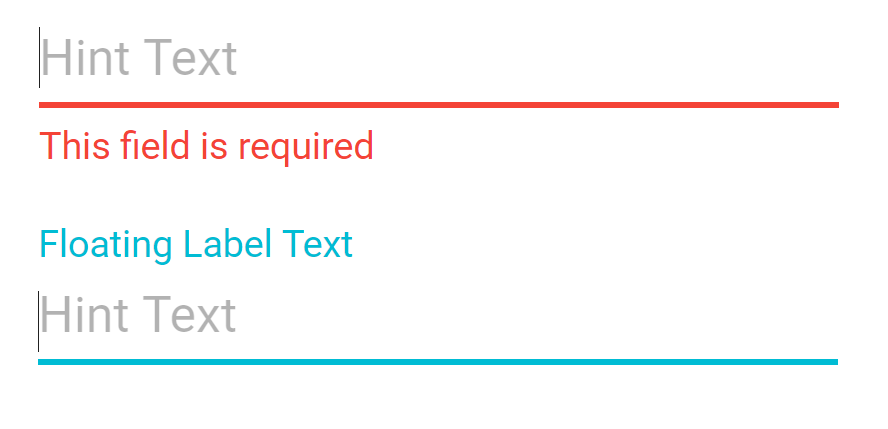
\includegraphics[width=0.5\textwidth]{img/materialui.png}
	\end{center}
    \caption{Príklad komponentov Text Field \parencite{materialui}.}
	\label{fig:materialui}
\end{figure}

React-Bootstrap poskytuje komponenty pre tvorbu responzívneho web dizajnu prostredníctvom populárnej knižnice Bootsrap, vytvorenej spoločnosťou Twitter. Predpokladaným zariadením, na ktorom sa bude rozhranie frontendu zobrazovať, sú monitory s vysokým rozlíšením, ale s využitím responzivity sa rozhranie prispôsobuje aj na obrazovky s menším rozlíšením, akými môžu byť staršie monitori s menšou uhlopriečkov, prípadne tablety.

\section{Architektúra}
\subsection{Kontajnerové a prezentačné komponenty}
Rozdelenie komponentov do kontajnerových a prezentačných je veľmi často používaný návrhový vzor pri vývoji aplikácie v Reacte. Kontajnerový komponent by mal obsahovať všetka aplikačnú logiku a prezentačný by mal obsahovať kód pre zobrazovanie dát, ktoré dostáva ako \texttt{props} od kontajnerového komponentu. Taktiež napríklad funkcie pre \texttt{event-handling} by mali byť definované v kontajnerovom komponente, ďalej predané ako \texttt{props} do prezentačného komponentu a v ňom priradené k určeným elementom.

Ďalším návrhovým vzorom je tvorba prezentačných komponentov bez využitia objektu \texttt{state}. Podľa toho sa rozdeľujú komponenty na \textit{statefull} a \textit{stateless} komponenty. Bez objektu \texttt{state} sa tak komponent správa ako funkcia, ktorá sa označuje pomenovaním \textit{pure function}. Znamená to, že pre rovnaké vstupné hodnoty (v prípade komponentov sú to \texttt{props}) sa vráti vždy rovnaká výstupná hodnota.

\subsection{Redux store}
Atribúty objektu \texttt{store} by mali byť rozčlenené podľa druhu dát, ktoré sú v nich uložené. Každý atribút má pridelený svoj reducer, v ktorom sa pri zmene dát vytvára nový stav, ktorý je následne priradený do príslušného atribútu. Iniciálny stav objektu vyzerá nasledovne:

\begin{lstlisting}[basicstyle=\small]
{
  routing: {
    ...
  },
  form: {
    ...
  }
  translate: {
    translations: []
  }
  dictionary: {
    dictionaries: [],
    dictionary: {
      name: '',
      words: []
    }
  }
}
\end{lstlisting}

Objekt \texttt{routing} obsahuje dáta, ktoré sú vytvorené pomocou knižnice React-router-redux. Dáta sa týkajú routingu v aplikácií, takže tam sú uložené napríklad parametre z URL alebo objekt \texttt{router}, ktorý obsahuje metódy pre manipuláciu s URL, takže sa dá pomocou nich vyvolať presmerovanie na inú stránku.

Objekt \texttt{form} je vytvorený externou knižnicou Redux-form, ktorá zjednodušuje prácu s formulármi. Ako bolo spomenuté v kapitole \ref{sec:oneway-binding}, v Reacte je potrebné vytvoriť handling pre zmeny dát v html elementoch typu input, ktoré bývajú súčasťou formulárov. To vykonáva práve táto knižnica. Pri zmenách v rôznych typoch inputov používa reduxové akcie a hodnoty s inputov ukladá do svojho \texttt{store}. Ten sa skladá z viacerych objektov, ktoré predstavujú jednotlivé formuláre v aplikácií, môže tak obsahovať atribúty s názvami \texttt{addWordForm}, \texttt{changeWordForm} a podobne, takže každý formulár má zapúzdrené svoje dáta.

Objekt \texttt{translate} obsahuje dáta využívané pri prekladaní slov. Pri každej požiadavke na preklad sa vrátené preklady uložia do pola \texttt{translations} a sú zobrazené na stránke.

Objekt \texttt{dictionary} obsahuje dáta využívané pri prekladaní slov. V poli \texttt{dictionaries} sa nachádza zoznam všetkých slovníkov dostupných na serveri. Tie sú potom využívané pri výbere konkrétnych slovníkov, v ktorých sa má slovo vyhľadávať na serveri. Ďalej sa využívajú na stánke so zonamom slovníkov. Vo vnorenom objekte \texttt{dictionary} sa nachádza konkrétny slovník obsahujúci všetky svoje slová. Pri vstúpení na stránku detailu slovníku sa konkrétny slovník načíta zo servera a jeho slová sú na stránke potom zobrazované.


\section{Implementácia}
Pre spustenie aplikácie v Reacte je potrebné mať nainštalované samotný modul React spolu s modulom React-dom a modul Webpack spolu s modulom Webpack-dev-server. Webpack slúži na vytvorenie finálneho javascriptového súbory, ktorý obsahuje build aplikácie. Tento súbor sa zvykne označovať ako bundle a je zdrojovým javascriptovým súborom pre stránku zobrazenú v internetovom prehliadači. Webpack-dev-server je server implementovaný v Node.js, ktorý slúži ako middleware pre správu súboru bundle \parencite{webpack}.

\subsection{Konfigurácia}
React využíva súbor \texttt{webpac.config.js} pre počiatočnú konfiguráciu Webpacku. Hlavné atribúty tejto konfigurácie sú \texttt{entry} - definuje vstupné moduly, z ktorých sa bude vytvárať finálny bundle súbor - ten je definovaný v atríbute \texttt{output}. Táto webová aplikácia má konkrétnu konfiguráciu definovanú nasledovne:

\begin{lstlisting}[basicstyle=\small]
module.exports = {  
  entry: {
    js: ['babel-polyfill', './src/index.js']
  },
  output: {
    filename: 'bundle.js',
  },
  ...
}
\end{lstlisting}

V prípade vstupného súboru \texttt{index.js} sa tento súbor ešte prekladá pomocou modulu Babel-polyfill, pretože pri implementácií aplikácie sú využité najnovšie prvky z Javascriptu, konkrétne ES7\footnote{Ecma Script 2016}, ktoré nie sú podporované v starších verziach prehliadačov. Zdrojový kód je tak vo výsledku preložený do Javascriptu s pôvodnými jazykovými formami, ktoré sú s väčšinou prehliadačov kompatibilné.

Ďalším prvkom konfigurácie je \texttt{devServer}, ktorý obsahuje konfiguráciu Webpack-dev-servera a aj proxy servera pre komunikáciu s API. V konfigurácii sa nastavujú aj rôzne moduly pre importovanie špecifických súborov, napríklad CSS štýlov v súboroch typu \texttt{.less}

\subsection{Preklad slov page}
\subsection{Praca so slovnikom page}

\chapter{Desktopový klient}
Desktopová aplikácia slúži pre vývojarávou ako pomoc pri práci so zdrojovými kódmi a je prispôsobená na rýchle vyhľadanie požadovaných prekladov. Je vytvorená tak, že poskytuje čo najjednoduchšie užívateľské rozhranie, aby vývojári nemuseli strácať čas so zaoberaním sa aplikáciou a mohli ju využívať čo najrýchlejsšie.

Desktopová aplikácia je vytvorená v programovacom jazyku C++ a využíva knižnicu GTK3+ pre tvorbu užívateľského rozhrania. Aby mohla byť synchronizovateľná, bola rozšírená o funkcionalitu pre komunikáciu so serverom, ďalej si ukladá lokálne vykonané zmeny nad slovníkmi a boli pridané nové prvky do GUI.

\section{Synchronizácia}
Aplikácia si ukladá zmeny rovnakým spôsobom ako server, má ku každému slovníku vytvorený ďalší súbor a zmeny sú vo formáte JSON. Musia sa zhodovať v štruktúre zmien zo servera, aby boli kompatibilné, takže obsahujú atribút \texttt{type}, ktorý nadobúda hodnoty \texttt{add} alebo \texttt{delete}, reprezentácia daných zmien je tiež rovnaká ako na serveri. Odlišujú sa však tým, že neobsahujú číslo revízie.

Aplikácia má uloženú práve jednu hodnotu revízie pre každý slovník, pričom tá sa mení iba pri synchronizácii. Vtedy sa posielajú lokálne zmeny a aplikácia dostane od servera novú hodnotu revízie spolu s novými zmenami od poslednej revízie. Prijaté zmeny sú všetky aplikované na synchronizovaný slovník a číslo revízie sa aktualizuje.

Prijaté zmeny nie je potrebné nijakým spôsobom spracovávať tak, ako je tomu na serveri a po ich aplikácii server predpokladá rovnaký konečný stav svojho a lokálneho slovníka v desktopovom klientovi. Novo vytvorené slovníky sa nesynchronizujù, ale novo sa vytvoria na serveri.

\subsection{Testy}
Súčasťou aplikácie sú aj unit testy, ktoré sú zamerané na synchronizáciu slovníkov. Testuje sa napríklad pripojenie na server, ale hlavnou úlohou testov je kontrola konečného stavu jednotlivých slovníkov po synchronizácií. Testuje sa tak primárne funkcionalita servera, ktorý má na starosti posielanie zmien pre klienta. Dôležité je, aby server posielal klientovy práve tie zmeny, ktoré klient nemá a aby boli slovníky po ich aplikácii konzistentné.

V testoch sa vždy vytvoria aspoň dva slovníky, ktoré sa na začiatku synchronizujú s nejakým iniciálnym zoznamom slov. Následne sa vykonávajú rôzne kombinácie operácií \textit{addWord}, \textit{changeWord} a \textit{deleteWord} vo všetkých slovníkoch. Potom sa slovníky opäť synchronizujú a porovnajú sa ich obsahy a revízie.

\begin{exmp}
\label{exmp:test}
Unit test na synchronizáciu slovníkov
\centering
\begin{lstlisting}[basicstyle=\small]
TEST_CASE("conflicts add-change", "[!hide][server]")
{
   Dict d1;
   d1.setName("testDictionary");
   d1.mOnline = true;
   d1.fill("base\n trBase\nword\n translation");
   d1.deleteFromServer(server).get();
   REQUIRE(d1.sync(server));

   d1.addWord("newWord", "newTranslationD1");
   d1.changeWord("word", "translationChangeD1");

   Dict d2;
   d2.mOnline = true;
   d2.setName("testDictionary");
   REQUIRE(d2.sync(server));

   d2.addWord("newWord", "newTranslationD2");
   d2.addWord("word", "translationAddD2");

   REQUIRE(d1.sync(server));
   REQUIRE(d2.sync(server));
   REQUIRE(d1.sync(server));

   L->info("d1: {}", *d1.getContens());
   L->info("d2: {}", *d2.getContens());

   REQUIRE(d1 == d2);
   REQUIRE(d1.getRevision() == d2.getRevision());
}
\end{lstlisting}
\end{exmp}

Na príklade \ref{exmp:test} je ukážka testu, ktorý sa zaoberá konfliktnými zmenami v slovníku. Vytvorené sú slovníky \texttt{d1} a \texttt{d2}, ktoré predstavujú rovnaké slovníky u dvoch rôznych klientov. Funkcia \texttt{d1.sync()} slovník synchronizuje, ak už je na serveri, ale ak nie je, tak ho vytvorí. Klient \texttt{d2} si tento slovník celý stiahne, kedže zatial na serveri nie sú uložené žiadne zmeny. Medzitým si klient \texttt{d1} aj \texttt{d2} uložia nové zmeny. Následne klient \texttt{d1} pošle svoje nové zmeny na server - \texttt{d1.sync()}, takže má uložené tieto slová:
\begin{lstlisting}[basicstyle=\small]
base: trBase
word: translationChangeD1
newWord: newTranslationD1
\end{lstlisting}

Po synchronizácii klienta \texttt{d2} má \texttt{d2} uložené tieto slová:

\begin{lstlisting}[basicstyle=\small]
base: trBase
newWord: newTranslationD2; newTranslationD1
word: translationAddD2; translationChangeD1
\end{lstlisting}

Po poslednej synchronizácií \texttt{d1} sa stiahnu nové zmeny od \texttt{d2} a \texttt{d1} tak obsahuje tieto slová:

\begin{lstlisting}[basicstyle=\small]
base: trBase
newWord: newTranslationD1; newTranslationD2
word: translationAddD1; translationChangeD2
\end{lstlisting}

Po synchronizácii sa slovníky porovnajú definovaným operátorom \texttt{==}, ktorý porovnáva jednotlivé slová a preklady, takže nezáleží na poradí slov v slovníkoch a prekladov v slovách. Taktiež revízie slovníka musia byť zhodné, keďže slovník \texttt{d1} už revíziu nezvyšoval, pretože neposielal žiadne nové zmeny.

\section{Užívateľské rozhranie}
Do užívateľskeho rozhrania bola pridaná možnosť pripojenia na server, cez ktorý sa majú slovníky synchronizovať. Táto možnosť sa nachádza v nastaveniach aplikácie a je znázornená na obrázku \ref{fig:desktop-settings}. Zakliknutím checkboxu \texttt{Synchronization server} sa dá zvoliť, či sa má aplikácia synchronizovať so serverom, a ak je táto možnosť zvolená, tak je možné zadať požadovanú URL, na ktorej sa server nachádza.
\begin{figure}
	\begin{center}
	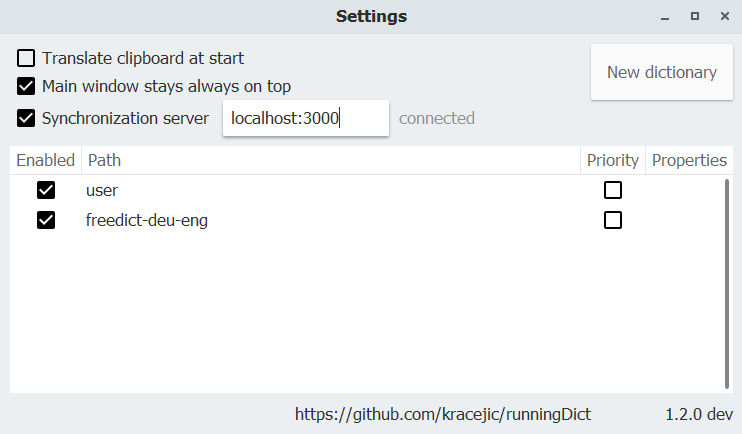
\includegraphics[width=0.8\textwidth]{img/desktop-settings.png}
	\end{center}
    \caption{Nastavenia aplikácie}
	\label{fig:desktop-settings}
\end{figure}

Na obrázku \ref{fig:desktop-ispublic} je dialódové okno pre vytvorenie nového slovníku. To obsahuje checkbox \texttt{Synchronized with server}, ktorým sa dá zvoliť možnosť, či slovník bude synchronizovaný alebo nie.
\begin{figure}
	\begin{center}
	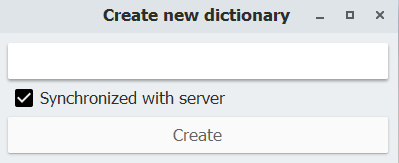
\includegraphics[width=0.6\textwidth]{img/desktop-ispublic.png}
	\end{center}
    \caption{Vytvorenie slovníka}
	\label{fig:desktop-ispublic}
\end{figure}

\chapter{Záver}
Táto diplomová práca sa zaoberala rozšírením desktopovej aplikácie prekladového slovníku o synchronizáciu slovníkov pomocou implementovaného servera a vytvorením webovej aplikácie slúžiacej ako frontend pre server. Vyvinutý softvér bude používaný v spoločnosti Siemens na súkromnej sieti. Webový klient bude slúžiť pre vývojárov, prípadne iných zamestnacov, ako užívateľské rozhranie prekladovej aplikácie.

Praktická časť zahŕňala návrh spôsobu synchronizácie slovníkov medzi desktopovou aplikáciou a serverom. Tá funguje pomocou ukladania zmien v podobe vykonaných operácií vo forme pridania alebo zmazania slova v offline režime. Rovnakým spôsobom sa zmeny ukladajú aj na serveri a po pripojení aplikácie do siete sa nové zmeny aplikujú na jej slovníky a jej zmeny na slovníky na serveri. Takýto spôsob synchronizácie je efektívnejší z pohľadu objemu zasielaných ako posielanie všetkých slov, ktorých môže byť v slovníku veľké množstvo.

Ďalším možným rozšírením backendu by mohla byť určitá forma autentizácie prístupu k vybraným slovníkom. V aktuálnom stave má každý užívateľ vo všetkých slovníkoch oprávnenie na čítanie aj zapisovanie dát. Užívateľ by si mohol vytvárať svoje privátne slovníky, do ktorých by mal prístup iba on, respektíve by mali ostatní užívatelia iba možnosť iba čítania dát zo slovníka. Najjednoduchším riešením by bolo slovníkom priradiť nejaký prístupový kód vo forme hesla, zložitejsím by bolo vytvoriť správu užívateľov. Oba prípady by si však vyžadovali rozšírenie všetkých softvérových častí - backendu, webového frontendu aj desktopového klienta.

Webový klient umožňuje všetky požadované operácie na prácu so slovníkmi - ich vytvorenie a odstránenie, v samotných slovníkoch potom pridanie, upravenie a mazanie slov. Taktiež je možné prekladať zadané slová podobne ako v desktopovej aplikácii. Existuje veľa možností rozšírenia frontendu, nová funkcionalita sa môže týkať rôznych filtrov alebo usporiadaní slov alebo slovníkov, ďalej môžu byť zobrazované rôzne štatistiky o zmenách v slovníku a podobne.


\chapter{Inserting the bibliography}
After linking a bibliography data\-base files to the document using
the \verb"\"\texttt{thesissetup\{bib\discretionary{=}{=}{=}%
\{\textit{file1},\textit{file2},\,\ldots\,\}\}} command, you can
start citing the entries. This is just dummy text
\parencite{borgman03} lightly sprinkled with citations
\parencite[p.~123]{greenberg98}. Several sources can be cited at
once: \cite{borgman03,greenberg98,thanh01}.
\citetitle{greenberg98} was written by \citeauthor{greenberg98} in
\citeyear{greenberg98}. We can also produce \textcite{greenberg98}%
\ or %% Let us define a compound command:
\def\citeauthoryear#1{(\textcite{#1},~\citeyear{#1})}%
\citeauthoryear{greenberg98}%
. The full bibliographic citation is:
\emph{\fullcite{greenberg98}}. We can easily insert a bibliographic
citation into the footnote\footfullcite{greenberg98}.

The \verb"\nocite" command will not generate any
output\nocite{muni}, but it will insert its arguments into
the bibliography. The \verb"\nocite{*}" command will insert all the
records in the bibliography database file into the bibliography.
Try uncommenting the command
%% \nocite{*}
and watch the bibliography section come apart at the seams.

When typesetting the document for the first time, citing a
\texttt{work} will expand to [\textbf{work}] and the
\verb"\printbibliography" command will produce no output. It is now
necessary to generate the bibliography by running \texttt{biber
\jobname.bcf} from the command line and then by typesetting the
document again twice. During the first run, the bibliography
section and the citations will be typeset, and in the second run,
the bibliography section will appear in the table of contents.

The \texttt{biber} command needs to be executed from within the
directory, where the \LaTeX\ source file is located. In Windows,
the command line can be opened in a directory by holding down the
\textsf{Shift} key and by clicking the right mouse button while
hovering the cursor over a directory.  Select the \textsf{Open
Command Window Here} option in the context menu that opens shortly
afterwards.

With online services -- such as Overleaf -- or when using an
automatic tool -- such as \LaTeX MK -- all commands are executed
automatically. When you omit the \verb"\printbibliography" command,
its location will be decided by the template.

  \printbibliography[heading=bibintoc] %% Print the bibliography.

\chapter{Inserting the index}
After using the \verb"\makeindex" macro and loading the
\texttt{makeidx} package that provides additional indexing
commands, index entries can be created by issuing the \verb"\index"
command. \index{dummy text|(}It is possible to create ranged index
entries, which will encompass a span of text.\index{dummy text|)}
To insert complex typographic material -- such as $\alpha$
\index{alpha@$\alpha$} or \TeX{} \index{TeX@\TeX} --
into the index, you need to specify a text string, which will
determine how the entry will be sorted. It is also possible to
create hierarchal entries. \index{vehicles!trucks}
\index{vehicles!speed cars}

After typesetting the document, it is necessary to generate the
index by running
\begin{center}%
  \texttt{texindy -I latex -C utf8 -L }$\langle$\textit{locale}%
  $\rangle$\texttt{ \jobname.idx}
\end{center}
from the command line, where $\langle$\textit{locale}$\rangle$
corresponds to the main locale of your thesis -- such as
\texttt{slovak}, and then typesetting the document again.

The \texttt{texindy} command needs to be executed from within the
directory, where the \LaTeX\ source file is located. In Windows,
the command line can be opened in a directory by holding down the
\textsf{Shift} key and by clicking the right mouse button while
hovering the cursor over a directory. Select the \textsf{Open Command
Window Here} option in the context menu that opens shortly
afterwards.

With online services -- such as Overleaf -- the commands are
executed automatically, although the locale may be erroneously
detected, or the \texttt{makeindex} tool (which is only able to
sort entries that contain digits and letters of the English
alphabet) may be used instead of \texttt{texindy}. In either case,
the index will be ill-sorted.

  \makeatletter\thesis@blocks@clear\makeatother
  \phantomsection %% Print the index and insert it into the
  \addcontentsline{toc}{chapter}{\indexname} %% table of contents.
  \printindex

\appendix %% Start the appendices.
\chapter{An appendix}
Here you can insert the appendices of your thesis.

\end{document}
